\documentclass[twoside]{book}

% Packages required by doxygen
\usepackage{fixltx2e}
\usepackage{calc}
\usepackage{doxygen}
\usepackage[export]{adjustbox} % also loads graphicx
\usepackage{graphicx}
\usepackage[utf8]{inputenc}
\usepackage{makeidx}
\usepackage{multicol}
\usepackage{multirow}
\PassOptionsToPackage{warn}{textcomp}
\usepackage{textcomp}
\usepackage[nointegrals]{wasysym}
\usepackage[table]{xcolor}

% Font selection
\usepackage[T1]{fontenc}
\usepackage[scaled=.90]{helvet}
\usepackage{courier}
\usepackage{amssymb}
\usepackage{sectsty}
\renewcommand{\familydefault}{\sfdefault}
\allsectionsfont{%
  \fontseries{bc}\selectfont%
  \color{darkgray}%
}
\renewcommand{\DoxyLabelFont}{%
  \fontseries{bc}\selectfont%
  \color{darkgray}%
}
\newcommand{\+}{\discretionary{\mbox{\scriptsize$\hookleftarrow$}}{}{}}

% Page & text layout
\usepackage{geometry}
\geometry{%
  a4paper,%
  top=2.5cm,%
  bottom=2.5cm,%
  left=2.5cm,%
  right=2.5cm%
}
\tolerance=750
\hfuzz=15pt
\hbadness=750
\setlength{\emergencystretch}{15pt}
\setlength{\parindent}{0cm}
\setlength{\parskip}{3ex plus 2ex minus 2ex}
\makeatletter
\renewcommand{\paragraph}{%
  \@startsection{paragraph}{4}{0ex}{-1.0ex}{1.0ex}{%
    \normalfont\normalsize\bfseries\SS@parafont%
  }%
}
\renewcommand{\subparagraph}{%
  \@startsection{subparagraph}{5}{0ex}{-1.0ex}{1.0ex}{%
    \normalfont\normalsize\bfseries\SS@subparafont%
  }%
}
\makeatother

% Headers & footers
\usepackage{fancyhdr}
\pagestyle{fancyplain}
\fancyhead[LE]{\fancyplain{}{\bfseries\thepage}}
\fancyhead[CE]{\fancyplain{}{}}
\fancyhead[RE]{\fancyplain{}{\bfseries\leftmark}}
\fancyhead[LO]{\fancyplain{}{\bfseries\rightmark}}
\fancyhead[CO]{\fancyplain{}{}}
\fancyhead[RO]{\fancyplain{}{\bfseries\thepage}}
\fancyfoot[LE]{\fancyplain{}{}}
\fancyfoot[CE]{\fancyplain{}{}}
\fancyfoot[RE]{\fancyplain{}{\bfseries\scriptsize Generated by Doxygen }}
\fancyfoot[LO]{\fancyplain{}{\bfseries\scriptsize Generated by Doxygen }}
\fancyfoot[CO]{\fancyplain{}{}}
\fancyfoot[RO]{\fancyplain{}{}}
\renewcommand{\footrulewidth}{0.4pt}
\renewcommand{\chaptermark}[1]{%
  \markboth{#1}{}%
}
\renewcommand{\sectionmark}[1]{%
  \markright{\thesection\ #1}%
}

% Indices & bibliography
\usepackage{natbib}
\usepackage[titles]{tocloft}
\setcounter{tocdepth}{3}
\setcounter{secnumdepth}{5}
\makeindex

% Hyperlinks (required, but should be loaded last)
\usepackage{ifpdf}
\ifpdf
  \usepackage[pdftex,pagebackref=true]{hyperref}
\else
  \usepackage[ps2pdf,pagebackref=true]{hyperref}
\fi
\hypersetup{%
  colorlinks=true,%
  linkcolor=blue,%
  citecolor=blue,%
  unicode%
}

% Custom commands
\newcommand{\clearemptydoublepage}{%
  \newpage{\pagestyle{empty}\cleardoublepage}%
}

\usepackage{caption}
\captionsetup{labelsep=space,justification=centering,font={bf},singlelinecheck=off,skip=4pt,position=top}

%===== C O N T E N T S =====

\begin{document}

% Titlepage & ToC
\hypersetup{pageanchor=false,
             bookmarksnumbered=true,
             pdfencoding=unicode
            }
\pagenumbering{roman}
\begin{titlepage}
\vspace*{7cm}
\begin{center}%
{\Large Assignment 2 }\\
\vspace*{1cm}
{\large Generated by Doxygen 1.8.11}\\
\end{center}
\end{titlepage}
\clearemptydoublepage
\tableofcontents
\clearemptydoublepage
\pagenumbering{arabic}
\hypersetup{pageanchor=true}

%--- Begin generated contents ---
\chapter{Namespace Index}
\section{Packages}
Here are the packages with brief descriptions (if available)\+:\begin{DoxyCompactList}
\item\contentsline{section}{\hyperlink{namespacecommandManager}{command\+Manager} }{\pageref{namespacecommandManager}}{}
\item\contentsline{section}{\hyperlink{namespacenoSleep}{no\+Sleep} }{\pageref{namespacenoSleep}}{}
\item\contentsline{section}{\hyperlink{namespaceroomDetector}{room\+Detector} }{\pageref{namespaceroomDetector}}{}
\item\contentsline{section}{\hyperlink{namespaceRooms}{Rooms} }{\pageref{namespaceRooms}}{}
\item\contentsline{section}{\hyperlink{namespacetrack}{track} }{\pageref{namespacetrack}}{}
\item\contentsline{section}{\hyperlink{namespaceUI}{UI} }{\pageref{namespaceUI}}{}
\end{DoxyCompactList}

\chapter{Hierarchical Index}
\section{Class Hierarchy}
This inheritance list is sorted roughly, but not completely, alphabetically\+:\begin{DoxyCompactList}
\item State\begin{DoxyCompactList}
\item \contentsline{section}{F\+S\+M.\+Normal}{\pageref{classFSM_1_1Normal}}{}
\item \contentsline{section}{F\+S\+M.\+Play}{\pageref{classFSM_1_1Play}}{}
\item \contentsline{section}{F\+S\+M.\+Sleep}{\pageref{classFSM_1_1Sleep}}{}
\item \contentsline{section}{F\+S\+Mplay.\+Normal}{\pageref{classFSMplay_1_1Normal}}{}
\item \contentsline{section}{F\+S\+Mplay.\+Play}{\pageref{classFSMplay_1_1Play}}{}
\item \contentsline{section}{F\+S\+Mplay.\+Sleep}{\pageref{classFSMplay_1_1Sleep}}{}
\item \contentsline{section}{state\+\_\+machine.\+Locked}{\pageref{classstate__machine_1_1Locked}}{}
\item \contentsline{section}{state\+\_\+machine.\+Unlocked}{\pageref{classstate__machine_1_1Unlocked}}{}
\end{DoxyCompactList}
\end{DoxyCompactList}

\chapter{Class Index}
\section{Class List}
Here are the classes, structs, unions and interfaces with brief descriptions\+:\begin{DoxyCompactList}
\item\contentsline{section}{\hyperlink{classcm2_1_1Find}{cm2.\+Find} }{\pageref{classcm2_1_1Find}}{}
\item\contentsline{section}{\hyperlink{classcommandManager_1_1Find}{command\+Manager.\+Find} }{\pageref{classcommandManager_1_1Find}}{}
\item\contentsline{section}{\hyperlink{classtimerProva_1_1lol}{timer\+Prova.\+lol} }{\pageref{classtimerProva_1_1lol}}{}
\item\contentsline{section}{\hyperlink{classcm2_1_1Normal}{cm2.\+Normal} }{\pageref{classcm2_1_1Normal}}{}
\item\contentsline{section}{\hyperlink{classcommandManager_1_1Normal}{command\+Manager.\+Normal} }{\pageref{classcommandManager_1_1Normal}}{}
\item\contentsline{section}{\hyperlink{classcommandManager_1_1Play}{command\+Manager.\+Play} }{\pageref{classcommandManager_1_1Play}}{}
\item\contentsline{section}{\hyperlink{classcm2_1_1Play}{cm2.\+Play} }{\pageref{classcm2_1_1Play}}{}
\item\contentsline{section}{\hyperlink{classroomDetector_1_1roomDetector}{room\+Detector.\+room\+Detector} \\*This class implements a subscriber to the camera topic of the robot and applies several open\+CV mask in order to recognise the color of the ball, then it send the detected color to the \hyperlink{namespacecommandManager}{command\+Manager} node }{\pageref{classroomDetector_1_1roomDetector}}{}
\item\contentsline{section}{\hyperlink{classroomsDetection_1_1roomDetector}{rooms\+Detection.\+room\+Detector} }{\pageref{classroomsDetection_1_1roomDetector}}{}
\item\contentsline{section}{\hyperlink{classRooms_1_1Rooms}{Rooms.\+Rooms} }{\pageref{classRooms_1_1Rooms}}{}
\item\contentsline{section}{\hyperlink{classcm2_1_1Sleep}{cm2.\+Sleep} }{\pageref{classcm2_1_1Sleep}}{}
\item\contentsline{section}{\hyperlink{classcommandManager_1_1Sleep}{command\+Manager.\+Sleep} }{\pageref{classcommandManager_1_1Sleep}}{}
\item\contentsline{section}{\hyperlink{classcommandManager_1_1Track}{command\+Manager.\+Track} }{\pageref{classcommandManager_1_1Track}}{}
\item\contentsline{section}{\hyperlink{classcm2_1_1Track}{cm2.\+Track} }{\pageref{classcm2_1_1Track}}{}
\item\contentsline{section}{\hyperlink{classtrackObj_1_1TrackAction}{track\+Obj.\+Track\+Action} \\*Class that implements the action server for tracking the ball }{\pageref{classtrackObj_1_1TrackAction}}{}
\item\contentsline{section}{\hyperlink{classtrack_1_1TrackAction}{track.\+Track\+Action} \\*Class that implements the action server for tracking the ball }{\pageref{classtrack_1_1TrackAction}}{}
\end{DoxyCompactList}

\chapter{File Index}
\section{File List}
Here is a list of all files with brief descriptions\+:\begin{DoxyCompactList}
\item\contentsline{section}{/home/experimental\+\_\+ws/src/final\+\_\+assignment/scripts/\hyperlink{cm2_8py}{cm2.\+py} }{\pageref{cm2_8py}}{}
\item\contentsline{section}{/home/experimental\+\_\+ws/src/final\+\_\+assignment/scripts/\hyperlink{cmd__smach_8py}{cmd\+\_\+smach.\+py} }{\pageref{cmd__smach_8py}}{}
\item\contentsline{section}{/home/experimental\+\_\+ws/src/final\+\_\+assignment/scripts/\hyperlink{commandManager_8py}{command\+Manager.\+py} \\*This script is a node which is the core of the entier project }{\pageref{commandManager_8py}}{}
\item\contentsline{section}{/home/experimental\+\_\+ws/src/final\+\_\+assignment/scripts/\hyperlink{roomDetector_8py}{room\+Detector.\+py} \\*This script implements the \hyperlink{namespaceroomDetector}{room\+Detector} class which basically is able to detect a ball and publish its color on the new\+Room topic }{\pageref{roomDetector_8py}}{}
\item\contentsline{section}{/home/experimental\+\_\+ws/src/final\+\_\+assignment/scripts/\hyperlink{Rooms_8py}{Rooms.\+py} \\*This script contains the \hyperlink{namespaceRooms}{Rooms} class, which implements a structure dedicated to the control and management of the rooms in a given environment }{\pageref{Rooms_8py}}{}
\item\contentsline{section}{/home/experimental\+\_\+ws/src/final\+\_\+assignment/scripts/\hyperlink{roomsDetection_8py}{rooms\+Detection.\+py} }{\pageref{roomsDetection_8py}}{}
\item\contentsline{section}{/home/experimental\+\_\+ws/src/final\+\_\+assignment/scripts/\hyperlink{timerProva_8py}{timer\+Prova.\+py} }{\pageref{timerProva_8py}}{}
\item\contentsline{section}{/home/experimental\+\_\+ws/src/final\+\_\+assignment/scripts/\hyperlink{track_8py}{track.\+py} \\*This script is an acttion server which takes a color of a ball in proximity of the robot and start to track it }{\pageref{track_8py}}{}
\item\contentsline{section}{/home/experimental\+\_\+ws/src/final\+\_\+assignment/scripts/\hyperlink{UI_8py}{U\+I.\+py} }{\pageref{UI_8py}}{}
\end{DoxyCompactList}

\chapter{Namespace Documentation}
\hypertarget{namespaceballDetection}{}\section{ball\+Detection Namespace Reference}
\label{namespaceballDetection}\index{ball\+Detection@{ball\+Detection}}
\subsection*{Classes}
\begin{DoxyCompactItemize}
\item 
class \hyperlink{classballDetection_1_1image__feature}{image\+\_\+feature}
\end{DoxyCompactItemize}
\subsection*{Functions}
\begin{DoxyCompactItemize}
\item 
def \hyperlink{namespaceballDetection_a8193b8aef394c20f60fadbaeacdafdc0}{main} (args)
\end{DoxyCompactItemize}
\subsection*{Variables}
\begin{DoxyCompactItemize}
\item 
bool \hyperlink{namespaceballDetection_a647c27a849ab906ef614cb5026275f43}{V\+E\+R\+B\+O\+SE} = False
\end{DoxyCompactItemize}


\subsection{Function Documentation}
\index{ball\+Detection@{ball\+Detection}!main@{main}}
\index{main@{main}!ball\+Detection@{ball\+Detection}}
\subsubsection[{\texorpdfstring{main(args)}{main(args)}}]{\setlength{\rightskip}{0pt plus 5cm}def ball\+Detection.\+main (
\begin{DoxyParamCaption}
\item[{}]{args}
\end{DoxyParamCaption}
)}\hypertarget{namespaceballDetection_a8193b8aef394c20f60fadbaeacdafdc0}{}\label{namespaceballDetection_a8193b8aef394c20f60fadbaeacdafdc0}
\begin{DoxyVerb}Initializes and cleanup ros node\end{DoxyVerb}
 

\subsection{Variable Documentation}
\index{ball\+Detection@{ball\+Detection}!V\+E\+R\+B\+O\+SE@{V\+E\+R\+B\+O\+SE}}
\index{V\+E\+R\+B\+O\+SE@{V\+E\+R\+B\+O\+SE}!ball\+Detection@{ball\+Detection}}
\subsubsection[{\texorpdfstring{V\+E\+R\+B\+O\+SE}{VERBOSE}}]{\setlength{\rightskip}{0pt plus 5cm}bool ball\+Detection.\+V\+E\+R\+B\+O\+SE = False}\hypertarget{namespaceballDetection_a647c27a849ab906ef614cb5026275f43}{}\label{namespaceballDetection_a647c27a849ab906ef614cb5026275f43}

\hypertarget{namespacecommandManager}{}\section{command\+Manager Namespace Reference}
\label{namespacecommandManager}\index{command\+Manager@{command\+Manager}}
\subsection*{Classes}
\begin{DoxyCompactItemize}
\item 
class \hyperlink{classcommandManager_1_1Find}{Find}
\item 
class \hyperlink{classcommandManager_1_1Normal}{Normal}
\item 
class \hyperlink{classcommandManager_1_1Play}{Play}
\item 
class \hyperlink{classcommandManager_1_1Sleep}{Sleep}
\item 
class \hyperlink{classcommandManager_1_1Track}{Track}
\end{DoxyCompactItemize}
\subsection*{Functions}
\begin{DoxyCompactItemize}
\item 
def \hyperlink{namespacecommandManager_a2310383d56755f0a09a75b1a92130e21}{U\+Icallback} (data)
\item 
def \hyperlink{namespacecommandManager_aa96fd2ed94c8c1168e09ced4015dcb1b}{new\+Room\+Detected} (color)
\item 
def \hyperlink{namespacecommandManager_af8e54858c65310eb1e131529bf200516}{move\+\_\+base\+\_\+go\+\_\+to} (x, y)
\item 
def \hyperlink{namespacecommandManager_ae8b570eb4bf393859bc74c9cb5fe125f}{main} ()
\end{DoxyCompactItemize}
\subsection*{Variables}
\begin{DoxyCompactItemize}
\item 
bool \hyperlink{namespacecommandManager_aecd980edd677f32e8693cbd21fa2c6eb}{P\+L\+AY} = False
\begin{DoxyCompactList}\small\item\em Flag which notify when the user types \textquotesingle{}play\textquotesingle{}. \end{DoxyCompactList}\item 
string \hyperlink{namespacecommandManager_ace76b1a89b584c851c50bc3ad66e1d69}{T\+A\+R\+G\+E\+T\+\_\+\+R\+O\+OM} = \char`\"{}None\char`\"{}
\begin{DoxyCompactList}\small\item\em Contains the desired room entered by the user. \end{DoxyCompactList}\item 
bool \hyperlink{namespacecommandManager_a6356544112d78464670ffb9af59bed1d}{N\+E\+W\+\_\+\+TR} = False
\begin{DoxyCompactList}\small\item\em Flag which notify when the command manager recives a new target room. \end{DoxyCompactList}\item 
bool \hyperlink{namespacecommandManager_a52e7163bf2cde17330107e6a2cf2f851}{N\+E\+W\+\_\+\+R\+O\+OM} = False
\begin{DoxyCompactList}\small\item\em new room detected \end{DoxyCompactList}\item 
bool \hyperlink{namespacecommandManager_afb1c5b8d9e6c746c82f4abf3fffe02a5}{R\+A\+N\+D\+OM} = True
\begin{DoxyCompactList}\small\item\em Random position generation flag. \end{DoxyCompactList}\item 
string \hyperlink{namespacecommandManager_ae945cfc4fe1632a6952debd7a67d9f3c}{C\+O\+L\+O\+R\+\_\+\+R\+O\+OM} = \char`\"{}None\char`\"{}
\begin{DoxyCompactList}\small\item\em color of the detected ball \end{DoxyCompactList}\item 
bool \hyperlink{namespacecommandManager_ad0728881cc70cfd3f8f5251b7b9af646}{F\+I\+N\+D\+\_\+\+M\+O\+DE} = False
\begin{DoxyCompactList}\small\item\em Flag to comeback into \hyperlink{classcommandManager_1_1Find}{Find} state when it\textquotesingle{}s necessary. \end{DoxyCompactList}\item 
\hyperlink{namespacecommandManager_ad81f5cdd9bf18b67989c77a2329b9e28}{client} = actionlib.\+Simple\+Action\+Client(\textquotesingle{}move\+\_\+base\textquotesingle{},Move\+Base\+Action)
\begin{DoxyCompactList}\small\item\em init the move\+\_\+base client \end{DoxyCompactList}\item 
\hyperlink{namespacecommandManager_a868809e1f6a79e7b7ce5ea405e978d48}{rooms} = \hyperlink{classRooms_1_1Rooms}{Rooms}()
\begin{DoxyCompactList}\small\item\em init the rooms environment \end{DoxyCompactList}\end{DoxyCompactItemize}


\subsection{Function Documentation}
\index{command\+Manager@{command\+Manager}!main@{main}}
\index{main@{main}!command\+Manager@{command\+Manager}}
\subsubsection[{\texorpdfstring{main()}{main()}}]{\setlength{\rightskip}{0pt plus 5cm}def command\+Manager.\+main (
\begin{DoxyParamCaption}
{}
\end{DoxyParamCaption}
)}\hypertarget{namespacecommandManager_ae8b570eb4bf393859bc74c9cb5fe125f}{}\label{namespacecommandManager_ae8b570eb4bf393859bc74c9cb5fe125f}
\index{command\+Manager@{command\+Manager}!move\+\_\+base\+\_\+go\+\_\+to@{move\+\_\+base\+\_\+go\+\_\+to}}
\index{move\+\_\+base\+\_\+go\+\_\+to@{move\+\_\+base\+\_\+go\+\_\+to}!command\+Manager@{command\+Manager}}
\subsubsection[{\texorpdfstring{move\+\_\+base\+\_\+go\+\_\+to(x, y)}{move_base_go_to(x, y)}}]{\setlength{\rightskip}{0pt plus 5cm}def command\+Manager.\+move\+\_\+base\+\_\+go\+\_\+to (
\begin{DoxyParamCaption}
\item[{}]{x, }
\item[{}]{y}
\end{DoxyParamCaption}
)}\hypertarget{namespacecommandManager_af8e54858c65310eb1e131529bf200516}{}\label{namespacecommandManager_af8e54858c65310eb1e131529bf200516}
\index{command\+Manager@{command\+Manager}!new\+Room\+Detected@{new\+Room\+Detected}}
\index{new\+Room\+Detected@{new\+Room\+Detected}!command\+Manager@{command\+Manager}}
\subsubsection[{\texorpdfstring{new\+Room\+Detected(color)}{newRoomDetected(color)}}]{\setlength{\rightskip}{0pt plus 5cm}def command\+Manager.\+new\+Room\+Detected (
\begin{DoxyParamCaption}
\item[{}]{color}
\end{DoxyParamCaption}
)}\hypertarget{namespacecommandManager_aa96fd2ed94c8c1168e09ced4015dcb1b}{}\label{namespacecommandManager_aa96fd2ed94c8c1168e09ced4015dcb1b}
\index{command\+Manager@{command\+Manager}!U\+Icallback@{U\+Icallback}}
\index{U\+Icallback@{U\+Icallback}!command\+Manager@{command\+Manager}}
\subsubsection[{\texorpdfstring{U\+Icallback(data)}{UIcallback(data)}}]{\setlength{\rightskip}{0pt plus 5cm}def command\+Manager.\+U\+Icallback (
\begin{DoxyParamCaption}
\item[{}]{data}
\end{DoxyParamCaption}
)}\hypertarget{namespacecommandManager_a2310383d56755f0a09a75b1a92130e21}{}\label{namespacecommandManager_a2310383d56755f0a09a75b1a92130e21}


\subsection{Variable Documentation}
\index{command\+Manager@{command\+Manager}!client@{client}}
\index{client@{client}!command\+Manager@{command\+Manager}}
\subsubsection[{\texorpdfstring{client}{client}}]{\setlength{\rightskip}{0pt plus 5cm}command\+Manager.\+client = actionlib.\+Simple\+Action\+Client(\textquotesingle{}move\+\_\+base\textquotesingle{},Move\+Base\+Action)}\hypertarget{namespacecommandManager_ad81f5cdd9bf18b67989c77a2329b9e28}{}\label{namespacecommandManager_ad81f5cdd9bf18b67989c77a2329b9e28}


init the move\+\_\+base client 

\index{command\+Manager@{command\+Manager}!C\+O\+L\+O\+R\+\_\+\+R\+O\+OM@{C\+O\+L\+O\+R\+\_\+\+R\+O\+OM}}
\index{C\+O\+L\+O\+R\+\_\+\+R\+O\+OM@{C\+O\+L\+O\+R\+\_\+\+R\+O\+OM}!command\+Manager@{command\+Manager}}
\subsubsection[{\texorpdfstring{C\+O\+L\+O\+R\+\_\+\+R\+O\+OM}{COLOR_ROOM}}]{\setlength{\rightskip}{0pt plus 5cm}string command\+Manager.\+C\+O\+L\+O\+R\+\_\+\+R\+O\+OM = \char`\"{}None\char`\"{}}\hypertarget{namespacecommandManager_ae945cfc4fe1632a6952debd7a67d9f3c}{}\label{namespacecommandManager_ae945cfc4fe1632a6952debd7a67d9f3c}


color of the detected ball 

\index{command\+Manager@{command\+Manager}!F\+I\+N\+D\+\_\+\+M\+O\+DE@{F\+I\+N\+D\+\_\+\+M\+O\+DE}}
\index{F\+I\+N\+D\+\_\+\+M\+O\+DE@{F\+I\+N\+D\+\_\+\+M\+O\+DE}!command\+Manager@{command\+Manager}}
\subsubsection[{\texorpdfstring{F\+I\+N\+D\+\_\+\+M\+O\+DE}{FIND_MODE}}]{\setlength{\rightskip}{0pt plus 5cm}bool command\+Manager.\+F\+I\+N\+D\+\_\+\+M\+O\+DE = False}\hypertarget{namespacecommandManager_ad0728881cc70cfd3f8f5251b7b9af646}{}\label{namespacecommandManager_ad0728881cc70cfd3f8f5251b7b9af646}


Flag to comeback into \hyperlink{classcommandManager_1_1Find}{Find} state when it\textquotesingle{}s necessary. 

\index{command\+Manager@{command\+Manager}!N\+E\+W\+\_\+\+R\+O\+OM@{N\+E\+W\+\_\+\+R\+O\+OM}}
\index{N\+E\+W\+\_\+\+R\+O\+OM@{N\+E\+W\+\_\+\+R\+O\+OM}!command\+Manager@{command\+Manager}}
\subsubsection[{\texorpdfstring{N\+E\+W\+\_\+\+R\+O\+OM}{NEW_ROOM}}]{\setlength{\rightskip}{0pt plus 5cm}bool command\+Manager.\+N\+E\+W\+\_\+\+R\+O\+OM = False}\hypertarget{namespacecommandManager_a52e7163bf2cde17330107e6a2cf2f851}{}\label{namespacecommandManager_a52e7163bf2cde17330107e6a2cf2f851}


new room detected 

\index{command\+Manager@{command\+Manager}!N\+E\+W\+\_\+\+TR@{N\+E\+W\+\_\+\+TR}}
\index{N\+E\+W\+\_\+\+TR@{N\+E\+W\+\_\+\+TR}!command\+Manager@{command\+Manager}}
\subsubsection[{\texorpdfstring{N\+E\+W\+\_\+\+TR}{NEW_TR}}]{\setlength{\rightskip}{0pt plus 5cm}bool command\+Manager.\+N\+E\+W\+\_\+\+TR = False}\hypertarget{namespacecommandManager_a6356544112d78464670ffb9af59bed1d}{}\label{namespacecommandManager_a6356544112d78464670ffb9af59bed1d}


Flag which notify when the command manager recives a new target room. 

\index{command\+Manager@{command\+Manager}!P\+L\+AY@{P\+L\+AY}}
\index{P\+L\+AY@{P\+L\+AY}!command\+Manager@{command\+Manager}}
\subsubsection[{\texorpdfstring{P\+L\+AY}{PLAY}}]{\setlength{\rightskip}{0pt plus 5cm}bool command\+Manager.\+P\+L\+AY = False}\hypertarget{namespacecommandManager_aecd980edd677f32e8693cbd21fa2c6eb}{}\label{namespacecommandManager_aecd980edd677f32e8693cbd21fa2c6eb}


Flag which notify when the user types \textquotesingle{}play\textquotesingle{}. 

\index{command\+Manager@{command\+Manager}!R\+A\+N\+D\+OM@{R\+A\+N\+D\+OM}}
\index{R\+A\+N\+D\+OM@{R\+A\+N\+D\+OM}!command\+Manager@{command\+Manager}}
\subsubsection[{\texorpdfstring{R\+A\+N\+D\+OM}{RANDOM}}]{\setlength{\rightskip}{0pt plus 5cm}bool command\+Manager.\+R\+A\+N\+D\+OM = True}\hypertarget{namespacecommandManager_afb1c5b8d9e6c746c82f4abf3fffe02a5}{}\label{namespacecommandManager_afb1c5b8d9e6c746c82f4abf3fffe02a5}


Random position generation flag. 

\index{command\+Manager@{command\+Manager}!rooms@{rooms}}
\index{rooms@{rooms}!command\+Manager@{command\+Manager}}
\subsubsection[{\texorpdfstring{rooms}{rooms}}]{\setlength{\rightskip}{0pt plus 5cm}command\+Manager.\+rooms = {\bf Rooms}()}\hypertarget{namespacecommandManager_a868809e1f6a79e7b7ce5ea405e978d48}{}\label{namespacecommandManager_a868809e1f6a79e7b7ce5ea405e978d48}


init the rooms environment 

\index{command\+Manager@{command\+Manager}!T\+A\+R\+G\+E\+T\+\_\+\+R\+O\+OM@{T\+A\+R\+G\+E\+T\+\_\+\+R\+O\+OM}}
\index{T\+A\+R\+G\+E\+T\+\_\+\+R\+O\+OM@{T\+A\+R\+G\+E\+T\+\_\+\+R\+O\+OM}!command\+Manager@{command\+Manager}}
\subsubsection[{\texorpdfstring{T\+A\+R\+G\+E\+T\+\_\+\+R\+O\+OM}{TARGET_ROOM}}]{\setlength{\rightskip}{0pt plus 5cm}string command\+Manager.\+T\+A\+R\+G\+E\+T\+\_\+\+R\+O\+OM = \char`\"{}None\char`\"{}}\hypertarget{namespacecommandManager_ace76b1a89b584c851c50bc3ad66e1d69}{}\label{namespacecommandManager_ace76b1a89b584c851c50bc3ad66e1d69}


Contains the desired room entered by the user. 


\hypertarget{namespacecvtest}{}\section{cvtest Namespace Reference}
\label{namespacecvtest}\index{cvtest@{cvtest}}
\subsection*{Classes}
\begin{DoxyCompactItemize}
\item 
class \hyperlink{classcvtest_1_1image__feature}{image\+\_\+feature}
\end{DoxyCompactItemize}
\subsection*{Functions}
\begin{DoxyCompactItemize}
\item 
def \hyperlink{namespacecvtest_ae154ff2084b8756ce8c727d4308e16e5}{main} (args)
\end{DoxyCompactItemize}
\subsection*{Variables}
\begin{DoxyCompactItemize}
\item 
bool \hyperlink{namespacecvtest_a77dc49644bd9f436671cd8f839604a45}{V\+E\+R\+B\+O\+SE} = False
\end{DoxyCompactItemize}


\subsection{Function Documentation}
\index{cvtest@{cvtest}!main@{main}}
\index{main@{main}!cvtest@{cvtest}}
\subsubsection[{\texorpdfstring{main(args)}{main(args)}}]{\setlength{\rightskip}{0pt plus 5cm}def cvtest.\+main (
\begin{DoxyParamCaption}
\item[{}]{args}
\end{DoxyParamCaption}
)}\hypertarget{namespacecvtest_ae154ff2084b8756ce8c727d4308e16e5}{}\label{namespacecvtest_ae154ff2084b8756ce8c727d4308e16e5}
\begin{DoxyVerb}Initializes and cleanup ros node\end{DoxyVerb}
 

\subsection{Variable Documentation}
\index{cvtest@{cvtest}!V\+E\+R\+B\+O\+SE@{V\+E\+R\+B\+O\+SE}}
\index{V\+E\+R\+B\+O\+SE@{V\+E\+R\+B\+O\+SE}!cvtest@{cvtest}}
\subsubsection[{\texorpdfstring{V\+E\+R\+B\+O\+SE}{VERBOSE}}]{\setlength{\rightskip}{0pt plus 5cm}bool cvtest.\+V\+E\+R\+B\+O\+SE = False}\hypertarget{namespacecvtest_a77dc49644bd9f436671cd8f839604a45}{}\label{namespacecvtest_a77dc49644bd9f436671cd8f839604a45}

\hypertarget{namespacego__to__point__ball}{}\section{go\+\_\+to\+\_\+point\+\_\+ball Namespace Reference}
\label{namespacego__to__point__ball}\index{go\+\_\+to\+\_\+point\+\_\+ball@{go\+\_\+to\+\_\+point\+\_\+ball}}
\subsection*{Functions}
\begin{DoxyCompactItemize}
\item 
def \hyperlink{namespacego__to__point__ball_a8b53c165c87e66822f50ab5daebc14dc}{clbk\+\_\+odom} (msg)
\item 
def \hyperlink{namespacego__to__point__ball_ac5839fd3601d15749a1e1a28939b2c68}{change\+\_\+state} (state)
\item 
def \hyperlink{namespacego__to__point__ball_aecbf76a67251ff6a3a0840bb61e1c581}{go\+\_\+straight\+\_\+ahead} (des\+\_\+pos)
\item 
def \hyperlink{namespacego__to__point__ball_ab92c8b4240f09ff0b5d960c748ade799}{done} ()
\item 
def \hyperlink{namespacego__to__point__ball_ab0e05a6be4adc81f80b5635d9bd692d1}{planning} (goal)
\item 
def \hyperlink{namespacego__to__point__ball_a4d4c016b6bb12c612710a2d39ade3465}{main} ()
\end{DoxyCompactItemize}
\subsection*{Variables}
\begin{DoxyCompactItemize}
\item 
\hyperlink{namespacego__to__point__ball_aa399e57145dd0af7eefcd5fab4174fe9}{position\+\_\+} = Point()
\item 
\hyperlink{namespacego__to__point__ball_a03f1d8b257a2ae3d173a18c3fc2f8602}{pose\+\_\+} = Pose()
\item 
int \hyperlink{namespacego__to__point__ball_a74d8ca28c507d35baf1ea8e8f9595a78}{yaw\+\_\+} = 0
\item 
int \hyperlink{namespacego__to__point__ball_a0028df70b94b4041119cceba5e5aa79d}{state\+\_\+} = 0
\item 
\hyperlink{namespacego__to__point__ball_ac81a8393fb253c9e0b7255f779f16884}{desired\+\_\+position\+\_\+} = Point()
\item 
int \hyperlink{namespacego__to__point__ball_acc228d72c1ee47a43061e3563ac20d5c}{yaw\+\_\+precision\+\_\+} = math.\+pi/9
\item 
int \hyperlink{namespacego__to__point__ball_a1985c69cf8534ba0bd2c6080f788a992}{yaw\+\_\+precision\+\_\+2\+\_\+} = math.\+pi/90
\item 
float \hyperlink{namespacego__to__point__ball_a9a02c8ca89a09909111972ec4fd317ca}{dist\+\_\+precision\+\_\+} = 0.\+1
\item 
float \hyperlink{namespacego__to__point__ball_aac67ecb6c41141092b1ccaba4b537afc}{kp\+\_\+a} = 3.\+0
\item 
float \hyperlink{namespacego__to__point__ball_aeb49969b88b7ca77d9abdeae42cb1964}{kp\+\_\+d} = 0.\+5
\item 
float \hyperlink{namespacego__to__point__ball_aa5173a26f3502ea035d7c563bbf1fb05}{ub\+\_\+a} = 0.\+6
\item 
float \hyperlink{namespacego__to__point__ball_ae6440cb2a8ea6e8e7d2327cb4cd12dd3}{lb\+\_\+a} = -\/0.\+5
\item 
float \hyperlink{namespacego__to__point__ball_a1dabe6f24f898fa6f5303959917de757}{ub\+\_\+d} = 2.\+0
\item 
float \hyperlink{namespacego__to__point__ball_a176944c73499ce72fa754c7e1a6d138d}{z\+\_\+back} = 0.\+25
\item 
\hyperlink{namespacego__to__point__ball_a00b95c7141b558cd4466ca89d7c81640}{pub} = None
\item 
\hyperlink{namespacego__to__point__ball_ae3016b9645d9bd2b863a34a30115a6af}{pubz} = None
\item 
\hyperlink{namespacego__to__point__ball_a9ac8c67ea55b320e5eb2bdf665173ffa}{act\+\_\+s} = None
\end{DoxyCompactItemize}


\subsection{Function Documentation}
\index{go\+\_\+to\+\_\+point\+\_\+ball@{go\+\_\+to\+\_\+point\+\_\+ball}!change\+\_\+state@{change\+\_\+state}}
\index{change\+\_\+state@{change\+\_\+state}!go\+\_\+to\+\_\+point\+\_\+ball@{go\+\_\+to\+\_\+point\+\_\+ball}}
\subsubsection[{\texorpdfstring{change\+\_\+state(state)}{change_state(state)}}]{\setlength{\rightskip}{0pt plus 5cm}def go\+\_\+to\+\_\+point\+\_\+ball.\+change\+\_\+state (
\begin{DoxyParamCaption}
\item[{}]{state}
\end{DoxyParamCaption}
)}\hypertarget{namespacego__to__point__ball_ac5839fd3601d15749a1e1a28939b2c68}{}\label{namespacego__to__point__ball_ac5839fd3601d15749a1e1a28939b2c68}
\index{go\+\_\+to\+\_\+point\+\_\+ball@{go\+\_\+to\+\_\+point\+\_\+ball}!clbk\+\_\+odom@{clbk\+\_\+odom}}
\index{clbk\+\_\+odom@{clbk\+\_\+odom}!go\+\_\+to\+\_\+point\+\_\+ball@{go\+\_\+to\+\_\+point\+\_\+ball}}
\subsubsection[{\texorpdfstring{clbk\+\_\+odom(msg)}{clbk_odom(msg)}}]{\setlength{\rightskip}{0pt plus 5cm}def go\+\_\+to\+\_\+point\+\_\+ball.\+clbk\+\_\+odom (
\begin{DoxyParamCaption}
\item[{}]{msg}
\end{DoxyParamCaption}
)}\hypertarget{namespacego__to__point__ball_a8b53c165c87e66822f50ab5daebc14dc}{}\label{namespacego__to__point__ball_a8b53c165c87e66822f50ab5daebc14dc}
\index{go\+\_\+to\+\_\+point\+\_\+ball@{go\+\_\+to\+\_\+point\+\_\+ball}!done@{done}}
\index{done@{done}!go\+\_\+to\+\_\+point\+\_\+ball@{go\+\_\+to\+\_\+point\+\_\+ball}}
\subsubsection[{\texorpdfstring{done()}{done()}}]{\setlength{\rightskip}{0pt plus 5cm}def go\+\_\+to\+\_\+point\+\_\+ball.\+done (
\begin{DoxyParamCaption}
{}
\end{DoxyParamCaption}
)}\hypertarget{namespacego__to__point__ball_ab92c8b4240f09ff0b5d960c748ade799}{}\label{namespacego__to__point__ball_ab92c8b4240f09ff0b5d960c748ade799}
\index{go\+\_\+to\+\_\+point\+\_\+ball@{go\+\_\+to\+\_\+point\+\_\+ball}!go\+\_\+straight\+\_\+ahead@{go\+\_\+straight\+\_\+ahead}}
\index{go\+\_\+straight\+\_\+ahead@{go\+\_\+straight\+\_\+ahead}!go\+\_\+to\+\_\+point\+\_\+ball@{go\+\_\+to\+\_\+point\+\_\+ball}}
\subsubsection[{\texorpdfstring{go\+\_\+straight\+\_\+ahead(des\+\_\+pos)}{go_straight_ahead(des_pos)}}]{\setlength{\rightskip}{0pt plus 5cm}def go\+\_\+to\+\_\+point\+\_\+ball.\+go\+\_\+straight\+\_\+ahead (
\begin{DoxyParamCaption}
\item[{}]{des\+\_\+pos}
\end{DoxyParamCaption}
)}\hypertarget{namespacego__to__point__ball_aecbf76a67251ff6a3a0840bb61e1c581}{}\label{namespacego__to__point__ball_aecbf76a67251ff6a3a0840bb61e1c581}
\index{go\+\_\+to\+\_\+point\+\_\+ball@{go\+\_\+to\+\_\+point\+\_\+ball}!main@{main}}
\index{main@{main}!go\+\_\+to\+\_\+point\+\_\+ball@{go\+\_\+to\+\_\+point\+\_\+ball}}
\subsubsection[{\texorpdfstring{main()}{main()}}]{\setlength{\rightskip}{0pt plus 5cm}def go\+\_\+to\+\_\+point\+\_\+ball.\+main (
\begin{DoxyParamCaption}
{}
\end{DoxyParamCaption}
)}\hypertarget{namespacego__to__point__ball_a4d4c016b6bb12c612710a2d39ade3465}{}\label{namespacego__to__point__ball_a4d4c016b6bb12c612710a2d39ade3465}
\index{go\+\_\+to\+\_\+point\+\_\+ball@{go\+\_\+to\+\_\+point\+\_\+ball}!planning@{planning}}
\index{planning@{planning}!go\+\_\+to\+\_\+point\+\_\+ball@{go\+\_\+to\+\_\+point\+\_\+ball}}
\subsubsection[{\texorpdfstring{planning(goal)}{planning(goal)}}]{\setlength{\rightskip}{0pt plus 5cm}def go\+\_\+to\+\_\+point\+\_\+ball.\+planning (
\begin{DoxyParamCaption}
\item[{}]{goal}
\end{DoxyParamCaption}
)}\hypertarget{namespacego__to__point__ball_ab0e05a6be4adc81f80b5635d9bd692d1}{}\label{namespacego__to__point__ball_ab0e05a6be4adc81f80b5635d9bd692d1}


\subsection{Variable Documentation}
\index{go\+\_\+to\+\_\+point\+\_\+ball@{go\+\_\+to\+\_\+point\+\_\+ball}!act\+\_\+s@{act\+\_\+s}}
\index{act\+\_\+s@{act\+\_\+s}!go\+\_\+to\+\_\+point\+\_\+ball@{go\+\_\+to\+\_\+point\+\_\+ball}}
\subsubsection[{\texorpdfstring{act\+\_\+s}{act_s}}]{\setlength{\rightskip}{0pt plus 5cm}go\+\_\+to\+\_\+point\+\_\+ball.\+act\+\_\+s = None}\hypertarget{namespacego__to__point__ball_a9ac8c67ea55b320e5eb2bdf665173ffa}{}\label{namespacego__to__point__ball_a9ac8c67ea55b320e5eb2bdf665173ffa}
\index{go\+\_\+to\+\_\+point\+\_\+ball@{go\+\_\+to\+\_\+point\+\_\+ball}!desired\+\_\+position\+\_\+@{desired\+\_\+position\+\_\+}}
\index{desired\+\_\+position\+\_\+@{desired\+\_\+position\+\_\+}!go\+\_\+to\+\_\+point\+\_\+ball@{go\+\_\+to\+\_\+point\+\_\+ball}}
\subsubsection[{\texorpdfstring{desired\+\_\+position\+\_\+}{desired_position_}}]{\setlength{\rightskip}{0pt plus 5cm}go\+\_\+to\+\_\+point\+\_\+ball.\+desired\+\_\+position\+\_\+ = Point()}\hypertarget{namespacego__to__point__ball_ac81a8393fb253c9e0b7255f779f16884}{}\label{namespacego__to__point__ball_ac81a8393fb253c9e0b7255f779f16884}
\index{go\+\_\+to\+\_\+point\+\_\+ball@{go\+\_\+to\+\_\+point\+\_\+ball}!dist\+\_\+precision\+\_\+@{dist\+\_\+precision\+\_\+}}
\index{dist\+\_\+precision\+\_\+@{dist\+\_\+precision\+\_\+}!go\+\_\+to\+\_\+point\+\_\+ball@{go\+\_\+to\+\_\+point\+\_\+ball}}
\subsubsection[{\texorpdfstring{dist\+\_\+precision\+\_\+}{dist_precision_}}]{\setlength{\rightskip}{0pt plus 5cm}float go\+\_\+to\+\_\+point\+\_\+ball.\+dist\+\_\+precision\+\_\+ = 0.\+1}\hypertarget{namespacego__to__point__ball_a9a02c8ca89a09909111972ec4fd317ca}{}\label{namespacego__to__point__ball_a9a02c8ca89a09909111972ec4fd317ca}
\index{go\+\_\+to\+\_\+point\+\_\+ball@{go\+\_\+to\+\_\+point\+\_\+ball}!kp\+\_\+a@{kp\+\_\+a}}
\index{kp\+\_\+a@{kp\+\_\+a}!go\+\_\+to\+\_\+point\+\_\+ball@{go\+\_\+to\+\_\+point\+\_\+ball}}
\subsubsection[{\texorpdfstring{kp\+\_\+a}{kp_a}}]{\setlength{\rightskip}{0pt plus 5cm}float go\+\_\+to\+\_\+point\+\_\+ball.\+kp\+\_\+a = 3.\+0}\hypertarget{namespacego__to__point__ball_aac67ecb6c41141092b1ccaba4b537afc}{}\label{namespacego__to__point__ball_aac67ecb6c41141092b1ccaba4b537afc}
\index{go\+\_\+to\+\_\+point\+\_\+ball@{go\+\_\+to\+\_\+point\+\_\+ball}!kp\+\_\+d@{kp\+\_\+d}}
\index{kp\+\_\+d@{kp\+\_\+d}!go\+\_\+to\+\_\+point\+\_\+ball@{go\+\_\+to\+\_\+point\+\_\+ball}}
\subsubsection[{\texorpdfstring{kp\+\_\+d}{kp_d}}]{\setlength{\rightskip}{0pt plus 5cm}float go\+\_\+to\+\_\+point\+\_\+ball.\+kp\+\_\+d = 0.\+5}\hypertarget{namespacego__to__point__ball_aeb49969b88b7ca77d9abdeae42cb1964}{}\label{namespacego__to__point__ball_aeb49969b88b7ca77d9abdeae42cb1964}
\index{go\+\_\+to\+\_\+point\+\_\+ball@{go\+\_\+to\+\_\+point\+\_\+ball}!lb\+\_\+a@{lb\+\_\+a}}
\index{lb\+\_\+a@{lb\+\_\+a}!go\+\_\+to\+\_\+point\+\_\+ball@{go\+\_\+to\+\_\+point\+\_\+ball}}
\subsubsection[{\texorpdfstring{lb\+\_\+a}{lb_a}}]{\setlength{\rightskip}{0pt plus 5cm}float go\+\_\+to\+\_\+point\+\_\+ball.\+lb\+\_\+a = -\/0.\+5}\hypertarget{namespacego__to__point__ball_ae6440cb2a8ea6e8e7d2327cb4cd12dd3}{}\label{namespacego__to__point__ball_ae6440cb2a8ea6e8e7d2327cb4cd12dd3}
\index{go\+\_\+to\+\_\+point\+\_\+ball@{go\+\_\+to\+\_\+point\+\_\+ball}!pose\+\_\+@{pose\+\_\+}}
\index{pose\+\_\+@{pose\+\_\+}!go\+\_\+to\+\_\+point\+\_\+ball@{go\+\_\+to\+\_\+point\+\_\+ball}}
\subsubsection[{\texorpdfstring{pose\+\_\+}{pose_}}]{\setlength{\rightskip}{0pt plus 5cm}go\+\_\+to\+\_\+point\+\_\+ball.\+pose\+\_\+ = Pose()}\hypertarget{namespacego__to__point__ball_a03f1d8b257a2ae3d173a18c3fc2f8602}{}\label{namespacego__to__point__ball_a03f1d8b257a2ae3d173a18c3fc2f8602}
\index{go\+\_\+to\+\_\+point\+\_\+ball@{go\+\_\+to\+\_\+point\+\_\+ball}!position\+\_\+@{position\+\_\+}}
\index{position\+\_\+@{position\+\_\+}!go\+\_\+to\+\_\+point\+\_\+ball@{go\+\_\+to\+\_\+point\+\_\+ball}}
\subsubsection[{\texorpdfstring{position\+\_\+}{position_}}]{\setlength{\rightskip}{0pt plus 5cm}go\+\_\+to\+\_\+point\+\_\+ball.\+position\+\_\+ = Point()}\hypertarget{namespacego__to__point__ball_aa399e57145dd0af7eefcd5fab4174fe9}{}\label{namespacego__to__point__ball_aa399e57145dd0af7eefcd5fab4174fe9}
\index{go\+\_\+to\+\_\+point\+\_\+ball@{go\+\_\+to\+\_\+point\+\_\+ball}!pub@{pub}}
\index{pub@{pub}!go\+\_\+to\+\_\+point\+\_\+ball@{go\+\_\+to\+\_\+point\+\_\+ball}}
\subsubsection[{\texorpdfstring{pub}{pub}}]{\setlength{\rightskip}{0pt plus 5cm}go\+\_\+to\+\_\+point\+\_\+ball.\+pub = None}\hypertarget{namespacego__to__point__ball_a00b95c7141b558cd4466ca89d7c81640}{}\label{namespacego__to__point__ball_a00b95c7141b558cd4466ca89d7c81640}
\index{go\+\_\+to\+\_\+point\+\_\+ball@{go\+\_\+to\+\_\+point\+\_\+ball}!pubz@{pubz}}
\index{pubz@{pubz}!go\+\_\+to\+\_\+point\+\_\+ball@{go\+\_\+to\+\_\+point\+\_\+ball}}
\subsubsection[{\texorpdfstring{pubz}{pubz}}]{\setlength{\rightskip}{0pt plus 5cm}go\+\_\+to\+\_\+point\+\_\+ball.\+pubz = None}\hypertarget{namespacego__to__point__ball_ae3016b9645d9bd2b863a34a30115a6af}{}\label{namespacego__to__point__ball_ae3016b9645d9bd2b863a34a30115a6af}
\index{go\+\_\+to\+\_\+point\+\_\+ball@{go\+\_\+to\+\_\+point\+\_\+ball}!state\+\_\+@{state\+\_\+}}
\index{state\+\_\+@{state\+\_\+}!go\+\_\+to\+\_\+point\+\_\+ball@{go\+\_\+to\+\_\+point\+\_\+ball}}
\subsubsection[{\texorpdfstring{state\+\_\+}{state_}}]{\setlength{\rightskip}{0pt plus 5cm}int go\+\_\+to\+\_\+point\+\_\+ball.\+state\+\_\+ = 0}\hypertarget{namespacego__to__point__ball_a0028df70b94b4041119cceba5e5aa79d}{}\label{namespacego__to__point__ball_a0028df70b94b4041119cceba5e5aa79d}
\index{go\+\_\+to\+\_\+point\+\_\+ball@{go\+\_\+to\+\_\+point\+\_\+ball}!ub\+\_\+a@{ub\+\_\+a}}
\index{ub\+\_\+a@{ub\+\_\+a}!go\+\_\+to\+\_\+point\+\_\+ball@{go\+\_\+to\+\_\+point\+\_\+ball}}
\subsubsection[{\texorpdfstring{ub\+\_\+a}{ub_a}}]{\setlength{\rightskip}{0pt plus 5cm}float go\+\_\+to\+\_\+point\+\_\+ball.\+ub\+\_\+a = 0.\+6}\hypertarget{namespacego__to__point__ball_aa5173a26f3502ea035d7c563bbf1fb05}{}\label{namespacego__to__point__ball_aa5173a26f3502ea035d7c563bbf1fb05}
\index{go\+\_\+to\+\_\+point\+\_\+ball@{go\+\_\+to\+\_\+point\+\_\+ball}!ub\+\_\+d@{ub\+\_\+d}}
\index{ub\+\_\+d@{ub\+\_\+d}!go\+\_\+to\+\_\+point\+\_\+ball@{go\+\_\+to\+\_\+point\+\_\+ball}}
\subsubsection[{\texorpdfstring{ub\+\_\+d}{ub_d}}]{\setlength{\rightskip}{0pt plus 5cm}float go\+\_\+to\+\_\+point\+\_\+ball.\+ub\+\_\+d = 2.\+0}\hypertarget{namespacego__to__point__ball_a1dabe6f24f898fa6f5303959917de757}{}\label{namespacego__to__point__ball_a1dabe6f24f898fa6f5303959917de757}
\index{go\+\_\+to\+\_\+point\+\_\+ball@{go\+\_\+to\+\_\+point\+\_\+ball}!yaw\+\_\+@{yaw\+\_\+}}
\index{yaw\+\_\+@{yaw\+\_\+}!go\+\_\+to\+\_\+point\+\_\+ball@{go\+\_\+to\+\_\+point\+\_\+ball}}
\subsubsection[{\texorpdfstring{yaw\+\_\+}{yaw_}}]{\setlength{\rightskip}{0pt plus 5cm}int go\+\_\+to\+\_\+point\+\_\+ball.\+yaw\+\_\+ = 0}\hypertarget{namespacego__to__point__ball_a74d8ca28c507d35baf1ea8e8f9595a78}{}\label{namespacego__to__point__ball_a74d8ca28c507d35baf1ea8e8f9595a78}
\index{go\+\_\+to\+\_\+point\+\_\+ball@{go\+\_\+to\+\_\+point\+\_\+ball}!yaw\+\_\+precision\+\_\+@{yaw\+\_\+precision\+\_\+}}
\index{yaw\+\_\+precision\+\_\+@{yaw\+\_\+precision\+\_\+}!go\+\_\+to\+\_\+point\+\_\+ball@{go\+\_\+to\+\_\+point\+\_\+ball}}
\subsubsection[{\texorpdfstring{yaw\+\_\+precision\+\_\+}{yaw_precision_}}]{\setlength{\rightskip}{0pt plus 5cm}int go\+\_\+to\+\_\+point\+\_\+ball.\+yaw\+\_\+precision\+\_\+ = math.\+pi/9}\hypertarget{namespacego__to__point__ball_acc228d72c1ee47a43061e3563ac20d5c}{}\label{namespacego__to__point__ball_acc228d72c1ee47a43061e3563ac20d5c}
\index{go\+\_\+to\+\_\+point\+\_\+ball@{go\+\_\+to\+\_\+point\+\_\+ball}!yaw\+\_\+precision\+\_\+2\+\_\+@{yaw\+\_\+precision\+\_\+2\+\_\+}}
\index{yaw\+\_\+precision\+\_\+2\+\_\+@{yaw\+\_\+precision\+\_\+2\+\_\+}!go\+\_\+to\+\_\+point\+\_\+ball@{go\+\_\+to\+\_\+point\+\_\+ball}}
\subsubsection[{\texorpdfstring{yaw\+\_\+precision\+\_\+2\+\_\+}{yaw_precision_2_}}]{\setlength{\rightskip}{0pt plus 5cm}int go\+\_\+to\+\_\+point\+\_\+ball.\+yaw\+\_\+precision\+\_\+2\+\_\+ = math.\+pi/90}\hypertarget{namespacego__to__point__ball_a1985c69cf8534ba0bd2c6080f788a992}{}\label{namespacego__to__point__ball_a1985c69cf8534ba0bd2c6080f788a992}
\index{go\+\_\+to\+\_\+point\+\_\+ball@{go\+\_\+to\+\_\+point\+\_\+ball}!z\+\_\+back@{z\+\_\+back}}
\index{z\+\_\+back@{z\+\_\+back}!go\+\_\+to\+\_\+point\+\_\+ball@{go\+\_\+to\+\_\+point\+\_\+ball}}
\subsubsection[{\texorpdfstring{z\+\_\+back}{z_back}}]{\setlength{\rightskip}{0pt plus 5cm}float go\+\_\+to\+\_\+point\+\_\+ball.\+z\+\_\+back = 0.\+25}\hypertarget{namespacego__to__point__ball_a176944c73499ce72fa754c7e1a6d138d}{}\label{namespacego__to__point__ball_a176944c73499ce72fa754c7e1a6d138d}

\hypertarget{namespacenavigation__action}{}\section{navigation\+\_\+action Namespace Reference}
\label{namespacenavigation__action}\index{navigation\+\_\+action@{navigation\+\_\+action}}
\subsection*{Functions}
\begin{DoxyCompactItemize}
\item 
def \hyperlink{namespacenavigation__action_a5843780136ed9def4e6c383d936ba03a}{clbk\+\_\+odom} (msg)
\begin{DoxyCompactList}\small\item\em callbacks \end{DoxyCompactList}\item 
def \hyperlink{namespacenavigation__action_a6d442ed74e58d2364dc836bf9070e294}{change\+\_\+state} (state)
\item 
def \hyperlink{namespacenavigation__action_a3d7bfdf0b3a4ceae6de2da2a2ca9216b}{normalize\+\_\+angle} (angle)
\item 
def \hyperlink{namespacenavigation__action_a66a81926b4ce0cf801c2a1e947dd2405}{fix\+\_\+yaw} (des\+\_\+pos)
\item 
def \hyperlink{namespacenavigation__action_a5984663372b3695a8566d9ab2b149728}{go\+\_\+straight\+\_\+ahead} (des\+\_\+pos)
\item 
def \hyperlink{namespacenavigation__action_a05d5b3c910a9327eceb1628bb0696e40}{done} ()
\item 
def \hyperlink{namespacenavigation__action_a2b437adab0003dc13c8703a505ba0640}{planning} (goal)
\begin{DoxyCompactList}\small\item\em callback of the action server \end{DoxyCompactList}\item 
def \hyperlink{namespacenavigation__action_a2203bb3f38935f8a73b3ef443dd4eec1}{main} ()
\end{DoxyCompactItemize}
\subsection*{Variables}
\begin{DoxyCompactItemize}
\item 
\hyperlink{namespacenavigation__action_aa53bb3e42cba75b4faece7677fdf8b1d}{position\+\_\+} = Point()
\begin{DoxyCompactList}\small\item\em robot state variables \end{DoxyCompactList}\item 
\hyperlink{namespacenavigation__action_ad906a8ccc8be8e7aac7662be3092c3b7}{pose\+\_\+} = Pose()
\item 
int \hyperlink{namespacenavigation__action_aa356f2a5947d276649face9801529b11}{yaw\+\_\+} = 0
\item 
int \hyperlink{namespacenavigation__action_ac6656a4827fb720e3c7a7224940626d2}{state\+\_\+} = 0
\begin{DoxyCompactList}\small\item\em machine state \end{DoxyCompactList}\item 
\hyperlink{namespacenavigation__action_a7ce69adc83a1ee3d37d5e3c6e0e72e32}{desired\+\_\+position\+\_\+} = Point()
\begin{DoxyCompactList}\small\item\em goal \end{DoxyCompactList}\item 
\hyperlink{namespacenavigation__action_a5258daa88a84ac3fae37a796753c3a6f}{z}
\item 
int \hyperlink{namespacenavigation__action_a405244594bb4eea456e03e5b095d3869}{yaw\+\_\+precision\+\_\+} = math.\+pi/9
\begin{DoxyCompactList}\small\item\em parameters \end{DoxyCompactList}\item 
int \hyperlink{namespacenavigation__action_a8ff0e6466c43c2a149fb09b9678d56bf}{yaw\+\_\+precision\+\_\+2\+\_\+} = math.\+pi/90
\item 
float \hyperlink{namespacenavigation__action_ae84ae6794723578c0bda3eb07d0f1387}{dist\+\_\+precision\+\_\+} = 0.\+1
\item 
float \hyperlink{namespacenavigation__action_a88d77c73344c091f0e27e30f34b149cc}{kp\+\_\+a} = 3.\+0
\item 
float \hyperlink{namespacenavigation__action_a34478a1ef79cccac170cae8f045a4018}{kp\+\_\+d} = 0.\+2
\begin{DoxyCompactList}\small\item\em In R\+OS Noetic, it may be necessary to change the sign of this proportional controller. \end{DoxyCompactList}\item 
float \hyperlink{namespacenavigation__action_a2949c425c74dfbe48d976545b4f4db9d}{ub\+\_\+a} = 0.\+6
\item 
float \hyperlink{namespacenavigation__action_aa1239a696c81960bbb147a15f3f3bd87}{lb\+\_\+a} = -\/0.\+5
\item 
float \hyperlink{namespacenavigation__action_aad75661fd33d72b125133a1898175d4b}{ub\+\_\+d} = 0.\+6
\item 
\hyperlink{namespacenavigation__action_a534f03fffb29fa18e1e2f01c2e99ac90}{pub} = None
\begin{DoxyCompactList}\small\item\em publisher \end{DoxyCompactList}\item 
\hyperlink{namespacenavigation__action_a0ff6186f4b199de2bb1fff9bdd2ad110}{act\+\_\+s} = None
\begin{DoxyCompactList}\small\item\em action\+\_\+server \end{DoxyCompactList}\item 
\hyperlink{namespacenavigation__action_a0d7ef71fc2d73b266e305aaca8a1330a}{joint\+\_\+pub} = rospy.\+Publisher(\char`\"{}joint\+\_\+head\+\_\+controller/command\char`\"{},Float64,queue\+\_\+size=1)
\begin{DoxyCompactList}\small\item\em Publisher. \end{DoxyCompactList}\end{DoxyCompactItemize}


\subsection{Function Documentation}
\index{navigation\+\_\+action@{navigation\+\_\+action}!change\+\_\+state@{change\+\_\+state}}
\index{change\+\_\+state@{change\+\_\+state}!navigation\+\_\+action@{navigation\+\_\+action}}
\subsubsection[{\texorpdfstring{change\+\_\+state(state)}{change_state(state)}}]{\setlength{\rightskip}{0pt plus 5cm}def navigation\+\_\+action.\+change\+\_\+state (
\begin{DoxyParamCaption}
\item[{}]{state}
\end{DoxyParamCaption}
)}\hypertarget{namespacenavigation__action_a6d442ed74e58d2364dc836bf9070e294}{}\label{namespacenavigation__action_a6d442ed74e58d2364dc836bf9070e294}
\index{navigation\+\_\+action@{navigation\+\_\+action}!clbk\+\_\+odom@{clbk\+\_\+odom}}
\index{clbk\+\_\+odom@{clbk\+\_\+odom}!navigation\+\_\+action@{navigation\+\_\+action}}
\subsubsection[{\texorpdfstring{clbk\+\_\+odom(msg)}{clbk_odom(msg)}}]{\setlength{\rightskip}{0pt plus 5cm}def navigation\+\_\+action.\+clbk\+\_\+odom (
\begin{DoxyParamCaption}
\item[{}]{msg}
\end{DoxyParamCaption}
)}\hypertarget{namespacenavigation__action_a5843780136ed9def4e6c383d936ba03a}{}\label{namespacenavigation__action_a5843780136ed9def4e6c383d936ba03a}


callbacks 

\index{navigation\+\_\+action@{navigation\+\_\+action}!done@{done}}
\index{done@{done}!navigation\+\_\+action@{navigation\+\_\+action}}
\subsubsection[{\texorpdfstring{done()}{done()}}]{\setlength{\rightskip}{0pt plus 5cm}def navigation\+\_\+action.\+done (
\begin{DoxyParamCaption}
{}
\end{DoxyParamCaption}
)}\hypertarget{namespacenavigation__action_a05d5b3c910a9327eceb1628bb0696e40}{}\label{namespacenavigation__action_a05d5b3c910a9327eceb1628bb0696e40}
\index{navigation\+\_\+action@{navigation\+\_\+action}!fix\+\_\+yaw@{fix\+\_\+yaw}}
\index{fix\+\_\+yaw@{fix\+\_\+yaw}!navigation\+\_\+action@{navigation\+\_\+action}}
\subsubsection[{\texorpdfstring{fix\+\_\+yaw(des\+\_\+pos)}{fix_yaw(des_pos)}}]{\setlength{\rightskip}{0pt plus 5cm}def navigation\+\_\+action.\+fix\+\_\+yaw (
\begin{DoxyParamCaption}
\item[{}]{des\+\_\+pos}
\end{DoxyParamCaption}
)}\hypertarget{namespacenavigation__action_a66a81926b4ce0cf801c2a1e947dd2405}{}\label{namespacenavigation__action_a66a81926b4ce0cf801c2a1e947dd2405}
\index{navigation\+\_\+action@{navigation\+\_\+action}!go\+\_\+straight\+\_\+ahead@{go\+\_\+straight\+\_\+ahead}}
\index{go\+\_\+straight\+\_\+ahead@{go\+\_\+straight\+\_\+ahead}!navigation\+\_\+action@{navigation\+\_\+action}}
\subsubsection[{\texorpdfstring{go\+\_\+straight\+\_\+ahead(des\+\_\+pos)}{go_straight_ahead(des_pos)}}]{\setlength{\rightskip}{0pt plus 5cm}def navigation\+\_\+action.\+go\+\_\+straight\+\_\+ahead (
\begin{DoxyParamCaption}
\item[{}]{des\+\_\+pos}
\end{DoxyParamCaption}
)}\hypertarget{namespacenavigation__action_a5984663372b3695a8566d9ab2b149728}{}\label{namespacenavigation__action_a5984663372b3695a8566d9ab2b149728}
\index{navigation\+\_\+action@{navigation\+\_\+action}!main@{main}}
\index{main@{main}!navigation\+\_\+action@{navigation\+\_\+action}}
\subsubsection[{\texorpdfstring{main()}{main()}}]{\setlength{\rightskip}{0pt plus 5cm}def navigation\+\_\+action.\+main (
\begin{DoxyParamCaption}
{}
\end{DoxyParamCaption}
)}\hypertarget{namespacenavigation__action_a2203bb3f38935f8a73b3ef443dd4eec1}{}\label{namespacenavigation__action_a2203bb3f38935f8a73b3ef443dd4eec1}
\index{navigation\+\_\+action@{navigation\+\_\+action}!normalize\+\_\+angle@{normalize\+\_\+angle}}
\index{normalize\+\_\+angle@{normalize\+\_\+angle}!navigation\+\_\+action@{navigation\+\_\+action}}
\subsubsection[{\texorpdfstring{normalize\+\_\+angle(angle)}{normalize_angle(angle)}}]{\setlength{\rightskip}{0pt plus 5cm}def navigation\+\_\+action.\+normalize\+\_\+angle (
\begin{DoxyParamCaption}
\item[{}]{angle}
\end{DoxyParamCaption}
)}\hypertarget{namespacenavigation__action_a3d7bfdf0b3a4ceae6de2da2a2ca9216b}{}\label{namespacenavigation__action_a3d7bfdf0b3a4ceae6de2da2a2ca9216b}
\index{navigation\+\_\+action@{navigation\+\_\+action}!planning@{planning}}
\index{planning@{planning}!navigation\+\_\+action@{navigation\+\_\+action}}
\subsubsection[{\texorpdfstring{planning(goal)}{planning(goal)}}]{\setlength{\rightskip}{0pt plus 5cm}def navigation\+\_\+action.\+planning (
\begin{DoxyParamCaption}
\item[{}]{goal}
\end{DoxyParamCaption}
)}\hypertarget{namespacenavigation__action_a2b437adab0003dc13c8703a505ba0640}{}\label{namespacenavigation__action_a2b437adab0003dc13c8703a505ba0640}


callback of the action server 



\subsection{Variable Documentation}
\index{navigation\+\_\+action@{navigation\+\_\+action}!act\+\_\+s@{act\+\_\+s}}
\index{act\+\_\+s@{act\+\_\+s}!navigation\+\_\+action@{navigation\+\_\+action}}
\subsubsection[{\texorpdfstring{act\+\_\+s}{act_s}}]{\setlength{\rightskip}{0pt plus 5cm}navigation\+\_\+action.\+act\+\_\+s = None}\hypertarget{namespacenavigation__action_a0ff6186f4b199de2bb1fff9bdd2ad110}{}\label{namespacenavigation__action_a0ff6186f4b199de2bb1fff9bdd2ad110}


action\+\_\+server 

\index{navigation\+\_\+action@{navigation\+\_\+action}!desired\+\_\+position\+\_\+@{desired\+\_\+position\+\_\+}}
\index{desired\+\_\+position\+\_\+@{desired\+\_\+position\+\_\+}!navigation\+\_\+action@{navigation\+\_\+action}}
\subsubsection[{\texorpdfstring{desired\+\_\+position\+\_\+}{desired_position_}}]{\setlength{\rightskip}{0pt plus 5cm}navigation\+\_\+action.\+desired\+\_\+position\+\_\+ = Point()}\hypertarget{namespacenavigation__action_a7ce69adc83a1ee3d37d5e3c6e0e72e32}{}\label{namespacenavigation__action_a7ce69adc83a1ee3d37d5e3c6e0e72e32}


goal 

\index{navigation\+\_\+action@{navigation\+\_\+action}!dist\+\_\+precision\+\_\+@{dist\+\_\+precision\+\_\+}}
\index{dist\+\_\+precision\+\_\+@{dist\+\_\+precision\+\_\+}!navigation\+\_\+action@{navigation\+\_\+action}}
\subsubsection[{\texorpdfstring{dist\+\_\+precision\+\_\+}{dist_precision_}}]{\setlength{\rightskip}{0pt plus 5cm}float navigation\+\_\+action.\+dist\+\_\+precision\+\_\+ = 0.\+1}\hypertarget{namespacenavigation__action_ae84ae6794723578c0bda3eb07d0f1387}{}\label{namespacenavigation__action_ae84ae6794723578c0bda3eb07d0f1387}
\index{navigation\+\_\+action@{navigation\+\_\+action}!joint\+\_\+pub@{joint\+\_\+pub}}
\index{joint\+\_\+pub@{joint\+\_\+pub}!navigation\+\_\+action@{navigation\+\_\+action}}
\subsubsection[{\texorpdfstring{joint\+\_\+pub}{joint_pub}}]{\setlength{\rightskip}{0pt plus 5cm}navigation\+\_\+action.\+joint\+\_\+pub = rospy.\+Publisher(\char`\"{}joint\+\_\+head\+\_\+controller/command\char`\"{},Float64,queue\+\_\+size=1)}\hypertarget{namespacenavigation__action_a0d7ef71fc2d73b266e305aaca8a1330a}{}\label{namespacenavigation__action_a0d7ef71fc2d73b266e305aaca8a1330a}


Publisher. 


\begin{DoxyParams}{Parameters}
{\em joint\+\_\+pub} & it allows to move the head of the robot \\
\hline
\end{DoxyParams}
\index{navigation\+\_\+action@{navigation\+\_\+action}!kp\+\_\+a@{kp\+\_\+a}}
\index{kp\+\_\+a@{kp\+\_\+a}!navigation\+\_\+action@{navigation\+\_\+action}}
\subsubsection[{\texorpdfstring{kp\+\_\+a}{kp_a}}]{\setlength{\rightskip}{0pt plus 5cm}float navigation\+\_\+action.\+kp\+\_\+a = 3.\+0}\hypertarget{namespacenavigation__action_a88d77c73344c091f0e27e30f34b149cc}{}\label{namespacenavigation__action_a88d77c73344c091f0e27e30f34b149cc}
\index{navigation\+\_\+action@{navigation\+\_\+action}!kp\+\_\+d@{kp\+\_\+d}}
\index{kp\+\_\+d@{kp\+\_\+d}!navigation\+\_\+action@{navigation\+\_\+action}}
\subsubsection[{\texorpdfstring{kp\+\_\+d}{kp_d}}]{\setlength{\rightskip}{0pt plus 5cm}float navigation\+\_\+action.\+kp\+\_\+d = 0.\+2}\hypertarget{namespacenavigation__action_a34478a1ef79cccac170cae8f045a4018}{}\label{namespacenavigation__action_a34478a1ef79cccac170cae8f045a4018}


In R\+OS Noetic, it may be necessary to change the sign of this proportional controller. 

\index{navigation\+\_\+action@{navigation\+\_\+action}!lb\+\_\+a@{lb\+\_\+a}}
\index{lb\+\_\+a@{lb\+\_\+a}!navigation\+\_\+action@{navigation\+\_\+action}}
\subsubsection[{\texorpdfstring{lb\+\_\+a}{lb_a}}]{\setlength{\rightskip}{0pt plus 5cm}float navigation\+\_\+action.\+lb\+\_\+a = -\/0.\+5}\hypertarget{namespacenavigation__action_aa1239a696c81960bbb147a15f3f3bd87}{}\label{namespacenavigation__action_aa1239a696c81960bbb147a15f3f3bd87}
\index{navigation\+\_\+action@{navigation\+\_\+action}!pose\+\_\+@{pose\+\_\+}}
\index{pose\+\_\+@{pose\+\_\+}!navigation\+\_\+action@{navigation\+\_\+action}}
\subsubsection[{\texorpdfstring{pose\+\_\+}{pose_}}]{\setlength{\rightskip}{0pt plus 5cm}navigation\+\_\+action.\+pose\+\_\+ = Pose()}\hypertarget{namespacenavigation__action_ad906a8ccc8be8e7aac7662be3092c3b7}{}\label{namespacenavigation__action_ad906a8ccc8be8e7aac7662be3092c3b7}
\index{navigation\+\_\+action@{navigation\+\_\+action}!position\+\_\+@{position\+\_\+}}
\index{position\+\_\+@{position\+\_\+}!navigation\+\_\+action@{navigation\+\_\+action}}
\subsubsection[{\texorpdfstring{position\+\_\+}{position_}}]{\setlength{\rightskip}{0pt plus 5cm}navigation\+\_\+action.\+position\+\_\+ = Point()}\hypertarget{namespacenavigation__action_aa53bb3e42cba75b4faece7677fdf8b1d}{}\label{namespacenavigation__action_aa53bb3e42cba75b4faece7677fdf8b1d}


robot state variables 

\index{navigation\+\_\+action@{navigation\+\_\+action}!pub@{pub}}
\index{pub@{pub}!navigation\+\_\+action@{navigation\+\_\+action}}
\subsubsection[{\texorpdfstring{pub}{pub}}]{\setlength{\rightskip}{0pt plus 5cm}navigation\+\_\+action.\+pub = None}\hypertarget{namespacenavigation__action_a534f03fffb29fa18e1e2f01c2e99ac90}{}\label{namespacenavigation__action_a534f03fffb29fa18e1e2f01c2e99ac90}


publisher 

\index{navigation\+\_\+action@{navigation\+\_\+action}!state\+\_\+@{state\+\_\+}}
\index{state\+\_\+@{state\+\_\+}!navigation\+\_\+action@{navigation\+\_\+action}}
\subsubsection[{\texorpdfstring{state\+\_\+}{state_}}]{\setlength{\rightskip}{0pt plus 5cm}int navigation\+\_\+action.\+state\+\_\+ = 0}\hypertarget{namespacenavigation__action_ac6656a4827fb720e3c7a7224940626d2}{}\label{namespacenavigation__action_ac6656a4827fb720e3c7a7224940626d2}


machine state 

\index{navigation\+\_\+action@{navigation\+\_\+action}!ub\+\_\+a@{ub\+\_\+a}}
\index{ub\+\_\+a@{ub\+\_\+a}!navigation\+\_\+action@{navigation\+\_\+action}}
\subsubsection[{\texorpdfstring{ub\+\_\+a}{ub_a}}]{\setlength{\rightskip}{0pt plus 5cm}float navigation\+\_\+action.\+ub\+\_\+a = 0.\+6}\hypertarget{namespacenavigation__action_a2949c425c74dfbe48d976545b4f4db9d}{}\label{namespacenavigation__action_a2949c425c74dfbe48d976545b4f4db9d}
\index{navigation\+\_\+action@{navigation\+\_\+action}!ub\+\_\+d@{ub\+\_\+d}}
\index{ub\+\_\+d@{ub\+\_\+d}!navigation\+\_\+action@{navigation\+\_\+action}}
\subsubsection[{\texorpdfstring{ub\+\_\+d}{ub_d}}]{\setlength{\rightskip}{0pt plus 5cm}float navigation\+\_\+action.\+ub\+\_\+d = 0.\+6}\hypertarget{namespacenavigation__action_aad75661fd33d72b125133a1898175d4b}{}\label{namespacenavigation__action_aad75661fd33d72b125133a1898175d4b}
\index{navigation\+\_\+action@{navigation\+\_\+action}!yaw\+\_\+@{yaw\+\_\+}}
\index{yaw\+\_\+@{yaw\+\_\+}!navigation\+\_\+action@{navigation\+\_\+action}}
\subsubsection[{\texorpdfstring{yaw\+\_\+}{yaw_}}]{\setlength{\rightskip}{0pt plus 5cm}int navigation\+\_\+action.\+yaw\+\_\+ = 0}\hypertarget{namespacenavigation__action_aa356f2a5947d276649face9801529b11}{}\label{namespacenavigation__action_aa356f2a5947d276649face9801529b11}
\index{navigation\+\_\+action@{navigation\+\_\+action}!yaw\+\_\+precision\+\_\+@{yaw\+\_\+precision\+\_\+}}
\index{yaw\+\_\+precision\+\_\+@{yaw\+\_\+precision\+\_\+}!navigation\+\_\+action@{navigation\+\_\+action}}
\subsubsection[{\texorpdfstring{yaw\+\_\+precision\+\_\+}{yaw_precision_}}]{\setlength{\rightskip}{0pt plus 5cm}int navigation\+\_\+action.\+yaw\+\_\+precision\+\_\+ = math.\+pi/9}\hypertarget{namespacenavigation__action_a405244594bb4eea456e03e5b095d3869}{}\label{namespacenavigation__action_a405244594bb4eea456e03e5b095d3869}


parameters 

\index{navigation\+\_\+action@{navigation\+\_\+action}!yaw\+\_\+precision\+\_\+2\+\_\+@{yaw\+\_\+precision\+\_\+2\+\_\+}}
\index{yaw\+\_\+precision\+\_\+2\+\_\+@{yaw\+\_\+precision\+\_\+2\+\_\+}!navigation\+\_\+action@{navigation\+\_\+action}}
\subsubsection[{\texorpdfstring{yaw\+\_\+precision\+\_\+2\+\_\+}{yaw_precision_2_}}]{\setlength{\rightskip}{0pt plus 5cm}int navigation\+\_\+action.\+yaw\+\_\+precision\+\_\+2\+\_\+ = math.\+pi/90}\hypertarget{namespacenavigation__action_a8ff0e6466c43c2a149fb09b9678d56bf}{}\label{namespacenavigation__action_a8ff0e6466c43c2a149fb09b9678d56bf}
\index{navigation\+\_\+action@{navigation\+\_\+action}!z@{z}}
\index{z@{z}!navigation\+\_\+action@{navigation\+\_\+action}}
\subsubsection[{\texorpdfstring{z}{z}}]{\setlength{\rightskip}{0pt plus 5cm}navigation\+\_\+action.\+z}\hypertarget{namespacenavigation__action_a5258daa88a84ac3fae37a796753c3a6f}{}\label{namespacenavigation__action_a5258daa88a84ac3fae37a796753c3a6f}

\chapter{Class Documentation}
\hypertarget{classballDetection_1_1image__feature}{}\section{ball\+Detection.\+image\+\_\+feature Class Reference}
\label{classballDetection_1_1image__feature}\index{ball\+Detection.\+image\+\_\+feature@{ball\+Detection.\+image\+\_\+feature}}
\subsection*{Public Member Functions}
\begin{DoxyCompactItemize}
\item 
def \hyperlink{classballDetection_1_1image__feature_a2de14dc8844b7778faaae3f1abc06064}{\+\_\+\+\_\+init\+\_\+\+\_\+} (self)
\item 
def \hyperlink{classballDetection_1_1image__feature_a7943b65b893b102334cb17c7bd3a1776}{Head\+State\+Callback} (self, data)
\item 
def \hyperlink{classballDetection_1_1image__feature_a7a61e6b57cc0b58d4ae4ca531fa8bbd0}{callback} (self, ros\+\_\+data)
\end{DoxyCompactItemize}
\subsection*{Public Attributes}
\begin{DoxyCompactItemize}
\item 
\hyperlink{classballDetection_1_1image__feature_a7873b5a7def0a26beb3bb7d08d51d5fe}{image\+\_\+pub}
\begin{DoxyCompactList}\small\item\em Publisher that send the processed and compressed images. \end{DoxyCompactList}\item 
\hyperlink{classballDetection_1_1image__feature_a5fa76faf1ca73df49668bbfbd6359ca6}{ball\+\_\+state\+\_\+pub}
\begin{DoxyCompactList}\small\item\em Publisher for send to the command manager information reguarding the ball and the corraction to apply to the robot. \end{DoxyCompactList}\item 
\hyperlink{classballDetection_1_1image__feature_a5097b180a748b724b36f9f77deddd703}{vel\+\_\+pub}
\begin{DoxyCompactList}\small\item\em Publisher to move the robot. \end{DoxyCompactList}\end{DoxyCompactItemize}
\subsection*{Static Public Attributes}
\begin{DoxyCompactItemize}
\item 
\hyperlink{classballDetection_1_1image__feature_ae58b2d15e5dc42eec2d49c6373f8e90b}{camera\+\_\+sub}
\begin{DoxyCompactList}\small\item\em To get the compressed images from the camera. \end{DoxyCompactList}\item 
\hyperlink{classballDetection_1_1image__feature_ac7ef080bc4849ca6a0fd93d6a4427381}{callback}
\item 
\hyperlink{classballDetection_1_1image__feature_a85c33da670bc2705900afcfa12cb2f66}{queue\+\_\+size}
\item 
\hyperlink{classballDetection_1_1image__feature_a90bb9d5a57637e7cef2ff093778b3182}{head\+\_\+state\+\_\+sub}
\begin{DoxyCompactList}\small\item\em Subscriber to the head\+\_\+state topic to know when the command manager has finished moving his head. \end{DoxyCompactList}\item 
\hyperlink{classballDetection_1_1image__feature_a17e637dcbb2639eab5dfefd9eccfb7d5}{Head\+State\+Callback}
\item 
\hyperlink{classballDetection_1_1image__feature_ac4aef32147d5a7ab2a5702b96d123ca5}{head\+State}
\begin{DoxyCompactList}\small\item\em Variable to check if the head is in the upright position. \end{DoxyCompactList}\item 
\hyperlink{classballDetection_1_1image__feature_ae7733d80f1a59b84036b204c44f1d594}{ball\+Reached}
\begin{DoxyCompactList}\small\item\em Variable that says whether the robot has reached the ball. \end{DoxyCompactList}\item 
tuple \hyperlink{classballDetection_1_1image__feature_a2b1d1abdc4e93d6a6eba6ba40f5a3f77}{green\+Lower} = (50, 50, 20)
\begin{DoxyCompactList}\small\item\em set colours bound \end{DoxyCompactList}\item 
tuple \hyperlink{classballDetection_1_1image__feature_a0a37e51a267a8f2e81abbbad3c120122}{green\+Upper} = (70, 255, 255)
\item 
\hyperlink{classballDetection_1_1image__feature_a192f6fe52f2e6067fac63cf7af3bebda}{blurred} = cv2.\+Gaussian\+Blur(image\+\_\+np, (11, 11), 0)
\item 
\hyperlink{classballDetection_1_1image__feature_a86c8b7e7581075179dea815950abb95f}{hsv} = cv2.\+cvt\+Color(\hyperlink{classballDetection_1_1image__feature_a192f6fe52f2e6067fac63cf7af3bebda}{blurred}, cv2.\+C\+O\+L\+O\+R\+\_\+\+B\+G\+R2\+H\+SV)
\item 
\hyperlink{classballDetection_1_1image__feature_ad659708b5d3ba7904aa0d4330266d41c}{mask} = cv2.\+in\+Range(\hyperlink{classballDetection_1_1image__feature_a86c8b7e7581075179dea815950abb95f}{hsv}, \hyperlink{classballDetection_1_1image__feature_a2b1d1abdc4e93d6a6eba6ba40f5a3f77}{green\+Lower}, \hyperlink{classballDetection_1_1image__feature_a0a37e51a267a8f2e81abbbad3c120122}{green\+Upper})
\item 
\hyperlink{classballDetection_1_1image__feature_a13f936766fe3bbfe466d4bef773bb4f9}{cnts}
\item 
\hyperlink{classballDetection_1_1image__feature_a3b6a3451dbb6f3643346969ea9af3670}{center} = None
\item 
\hyperlink{classballDetection_1_1image__feature_a0ffd02f437ce41c517d2c870c059739b}{c} = max(\hyperlink{classballDetection_1_1image__feature_a13f936766fe3bbfe466d4bef773bb4f9}{cnts}, key=cv2.\+contour\+Area)
\item 
\hyperlink{classballDetection_1_1image__feature_a370e9015a86097812e323a9e18607c04}{radius}
\item 
\hyperlink{classballDetection_1_1image__feature_a45bb9e555b09541234f1724df7424e90}{M} = cv2.\+moments(\hyperlink{classballDetection_1_1image__feature_a0ffd02f437ce41c517d2c870c059739b}{c})
\item 
tuple \hyperlink{classballDetection_1_1image__feature_a7decaea2748c245d5940ea2f267a4cfc}{center} = (int(\hyperlink{classballDetection_1_1image__feature_a45bb9e555b09541234f1724df7424e90}{M}\mbox{[}\char`\"{}m10\char`\"{}\mbox{]} / M\mbox{[}\char`\"{}m00\char`\"{}\mbox{]}), int(\hyperlink{classballDetection_1_1image__feature_a45bb9e555b09541234f1724df7424e90}{M}\mbox{[}\char`\"{}m01\char`\"{}\mbox{]} / M\mbox{[}\char`\"{}m00\char`\"{}\mbox{]}))
\item 
\hyperlink{classballDetection_1_1image__feature_a3217e5c3695187fcf57a71915908e2fa}{msg} = Ball\+\_\+state()
\item 
\hyperlink{classballDetection_1_1image__feature_a60c51ba153ca9be2cb0231850f9a06bb}{ball\+Detected}
\begin{DoxyCompactList}\small\item\em Field of the R\+OS msg Ball\+\_\+state. \end{DoxyCompactList}\item 
\hyperlink{classballDetection_1_1image__feature_a871d6d1a252f9af8acb9695a52d2a465}{vel} = Twist()
\item 
\hyperlink{classballDetection_1_1image__feature_aae155697ae683625f463cb1839364095}{z}
\item 
\hyperlink{classballDetection_1_1image__feature_aaaf308b2b30ca2a20253d5e7ec3007b6}{x}
\end{DoxyCompactItemize}


\subsection{Constructor \& Destructor Documentation}
\index{ball\+Detection\+::image\+\_\+feature@{ball\+Detection\+::image\+\_\+feature}!\+\_\+\+\_\+init\+\_\+\+\_\+@{\+\_\+\+\_\+init\+\_\+\+\_\+}}
\index{\+\_\+\+\_\+init\+\_\+\+\_\+@{\+\_\+\+\_\+init\+\_\+\+\_\+}!ball\+Detection\+::image\+\_\+feature@{ball\+Detection\+::image\+\_\+feature}}
\subsubsection[{\texorpdfstring{\+\_\+\+\_\+init\+\_\+\+\_\+(self)}{__init__(self)}}]{\setlength{\rightskip}{0pt plus 5cm}def ball\+Detection.\+image\+\_\+feature.\+\_\+\+\_\+init\+\_\+\+\_\+ (
\begin{DoxyParamCaption}
\item[{}]{self}
\end{DoxyParamCaption}
)}\hypertarget{classballDetection_1_1image__feature_a2de14dc8844b7778faaae3f1abc06064}{}\label{classballDetection_1_1image__feature_a2de14dc8844b7778faaae3f1abc06064}
\begin{DoxyVerb}Initialize ros publisher, ros subscriber\end{DoxyVerb}
 

\subsection{Member Function Documentation}
\index{ball\+Detection\+::image\+\_\+feature@{ball\+Detection\+::image\+\_\+feature}!callback@{callback}}
\index{callback@{callback}!ball\+Detection\+::image\+\_\+feature@{ball\+Detection\+::image\+\_\+feature}}
\subsubsection[{\texorpdfstring{callback(self, ros\+\_\+data)}{callback(self, ros_data)}}]{\setlength{\rightskip}{0pt plus 5cm}def ball\+Detection.\+image\+\_\+feature.\+callback (
\begin{DoxyParamCaption}
\item[{}]{self, }
\item[{}]{ros\+\_\+data}
\end{DoxyParamCaption}
)}\hypertarget{classballDetection_1_1image__feature_a7a61e6b57cc0b58d4ae4ca531fa8bbd0}{}\label{classballDetection_1_1image__feature_a7a61e6b57cc0b58d4ae4ca531fa8bbd0}
\begin{DoxyVerb}Callback function of subscribed "camera_sub" topic which implements 
the whole Computer Vision algorithm  \end{DoxyVerb}
 \index{ball\+Detection\+::image\+\_\+feature@{ball\+Detection\+::image\+\_\+feature}!Head\+State\+Callback@{Head\+State\+Callback}}
\index{Head\+State\+Callback@{Head\+State\+Callback}!ball\+Detection\+::image\+\_\+feature@{ball\+Detection\+::image\+\_\+feature}}
\subsubsection[{\texorpdfstring{Head\+State\+Callback(self, data)}{HeadStateCallback(self, data)}}]{\setlength{\rightskip}{0pt plus 5cm}def ball\+Detection.\+image\+\_\+feature.\+Head\+State\+Callback (
\begin{DoxyParamCaption}
\item[{}]{self, }
\item[{}]{data}
\end{DoxyParamCaption}
)}\hypertarget{classballDetection_1_1image__feature_a7943b65b893b102334cb17c7bd3a1776}{}\label{classballDetection_1_1image__feature_a7943b65b893b102334cb17c7bd3a1776}
\begin{DoxyVerb}Callback function of subscribed "head_state" topic.
     This function updates the "headState" value\end{DoxyVerb}
 

\subsection{Member Data Documentation}
\index{ball\+Detection\+::image\+\_\+feature@{ball\+Detection\+::image\+\_\+feature}!ball\+\_\+state\+\_\+pub@{ball\+\_\+state\+\_\+pub}}
\index{ball\+\_\+state\+\_\+pub@{ball\+\_\+state\+\_\+pub}!ball\+Detection\+::image\+\_\+feature@{ball\+Detection\+::image\+\_\+feature}}
\subsubsection[{\texorpdfstring{ball\+\_\+state\+\_\+pub}{ball_state_pub}}]{\setlength{\rightskip}{0pt plus 5cm}ball\+Detection.\+image\+\_\+feature.\+ball\+\_\+state\+\_\+pub}\hypertarget{classballDetection_1_1image__feature_a5fa76faf1ca73df49668bbfbd6359ca6}{}\label{classballDetection_1_1image__feature_a5fa76faf1ca73df49668bbfbd6359ca6}


Publisher for send to the command manager information reguarding the ball and the corraction to apply to the robot. 

\index{ball\+Detection\+::image\+\_\+feature@{ball\+Detection\+::image\+\_\+feature}!ball\+Detected@{ball\+Detected}}
\index{ball\+Detected@{ball\+Detected}!ball\+Detection\+::image\+\_\+feature@{ball\+Detection\+::image\+\_\+feature}}
\subsubsection[{\texorpdfstring{ball\+Detected}{ballDetected}}]{\setlength{\rightskip}{0pt plus 5cm}ball\+Detection.\+image\+\_\+feature.\+ball\+Detected\hspace{0.3cm}{\ttfamily [static]}}\hypertarget{classballDetection_1_1image__feature_a60c51ba153ca9be2cb0231850f9a06bb}{}\label{classballDetection_1_1image__feature_a60c51ba153ca9be2cb0231850f9a06bb}


Field of the R\+OS msg Ball\+\_\+state. 

\index{ball\+Detection\+::image\+\_\+feature@{ball\+Detection\+::image\+\_\+feature}!ball\+Reached@{ball\+Reached}}
\index{ball\+Reached@{ball\+Reached}!ball\+Detection\+::image\+\_\+feature@{ball\+Detection\+::image\+\_\+feature}}
\subsubsection[{\texorpdfstring{ball\+Reached}{ballReached}}]{\setlength{\rightskip}{0pt plus 5cm}ball\+Detection.\+image\+\_\+feature.\+ball\+Reached\hspace{0.3cm}{\ttfamily [static]}}\hypertarget{classballDetection_1_1image__feature_ae7733d80f1a59b84036b204c44f1d594}{}\label{classballDetection_1_1image__feature_ae7733d80f1a59b84036b204c44f1d594}


Variable that says whether the robot has reached the ball. 

\index{ball\+Detection\+::image\+\_\+feature@{ball\+Detection\+::image\+\_\+feature}!blurred@{blurred}}
\index{blurred@{blurred}!ball\+Detection\+::image\+\_\+feature@{ball\+Detection\+::image\+\_\+feature}}
\subsubsection[{\texorpdfstring{blurred}{blurred}}]{\setlength{\rightskip}{0pt plus 5cm}ball\+Detection.\+image\+\_\+feature.\+blurred = cv2.\+Gaussian\+Blur(image\+\_\+np, (11, 11), 0)\hspace{0.3cm}{\ttfamily [static]}}\hypertarget{classballDetection_1_1image__feature_a192f6fe52f2e6067fac63cf7af3bebda}{}\label{classballDetection_1_1image__feature_a192f6fe52f2e6067fac63cf7af3bebda}
\index{ball\+Detection\+::image\+\_\+feature@{ball\+Detection\+::image\+\_\+feature}!c@{c}}
\index{c@{c}!ball\+Detection\+::image\+\_\+feature@{ball\+Detection\+::image\+\_\+feature}}
\subsubsection[{\texorpdfstring{c}{c}}]{\setlength{\rightskip}{0pt plus 5cm}ball\+Detection.\+image\+\_\+feature.\+c = max({\bf cnts}, key=cv2.\+contour\+Area)\hspace{0.3cm}{\ttfamily [static]}}\hypertarget{classballDetection_1_1image__feature_a0ffd02f437ce41c517d2c870c059739b}{}\label{classballDetection_1_1image__feature_a0ffd02f437ce41c517d2c870c059739b}
\index{ball\+Detection\+::image\+\_\+feature@{ball\+Detection\+::image\+\_\+feature}!callback@{callback}}
\index{callback@{callback}!ball\+Detection\+::image\+\_\+feature@{ball\+Detection\+::image\+\_\+feature}}
\subsubsection[{\texorpdfstring{callback}{callback}}]{\setlength{\rightskip}{0pt plus 5cm}ball\+Detection.\+image\+\_\+feature.\+callback\hspace{0.3cm}{\ttfamily [static]}}\hypertarget{classballDetection_1_1image__feature_ac7ef080bc4849ca6a0fd93d6a4427381}{}\label{classballDetection_1_1image__feature_ac7ef080bc4849ca6a0fd93d6a4427381}
\index{ball\+Detection\+::image\+\_\+feature@{ball\+Detection\+::image\+\_\+feature}!camera\+\_\+sub@{camera\+\_\+sub}}
\index{camera\+\_\+sub@{camera\+\_\+sub}!ball\+Detection\+::image\+\_\+feature@{ball\+Detection\+::image\+\_\+feature}}
\subsubsection[{\texorpdfstring{camera\+\_\+sub}{camera_sub}}]{\setlength{\rightskip}{0pt plus 5cm}ball\+Detection.\+image\+\_\+feature.\+camera\+\_\+sub\hspace{0.3cm}{\ttfamily [static]}}\hypertarget{classballDetection_1_1image__feature_ae58b2d15e5dc42eec2d49c6373f8e90b}{}\label{classballDetection_1_1image__feature_ae58b2d15e5dc42eec2d49c6373f8e90b}


To get the compressed images from the camera. 

\index{ball\+Detection\+::image\+\_\+feature@{ball\+Detection\+::image\+\_\+feature}!center@{center}}
\index{center@{center}!ball\+Detection\+::image\+\_\+feature@{ball\+Detection\+::image\+\_\+feature}}
\subsubsection[{\texorpdfstring{center}{center}}]{\setlength{\rightskip}{0pt plus 5cm}ball\+Detection.\+image\+\_\+feature.\+center = None\hspace{0.3cm}{\ttfamily [static]}}\hypertarget{classballDetection_1_1image__feature_a3b6a3451dbb6f3643346969ea9af3670}{}\label{classballDetection_1_1image__feature_a3b6a3451dbb6f3643346969ea9af3670}
\index{ball\+Detection\+::image\+\_\+feature@{ball\+Detection\+::image\+\_\+feature}!center@{center}}
\index{center@{center}!ball\+Detection\+::image\+\_\+feature@{ball\+Detection\+::image\+\_\+feature}}
\subsubsection[{\texorpdfstring{center}{center}}]{\setlength{\rightskip}{0pt plus 5cm}tuple ball\+Detection.\+image\+\_\+feature.\+center = (int({\bf M}\mbox{[}\char`\"{}m10\char`\"{}\mbox{]} / M\mbox{[}\char`\"{}m00\char`\"{}\mbox{]}), int({\bf M}\mbox{[}\char`\"{}m01\char`\"{}\mbox{]} / M\mbox{[}\char`\"{}m00\char`\"{}\mbox{]}))\hspace{0.3cm}{\ttfamily [static]}}\hypertarget{classballDetection_1_1image__feature_a7decaea2748c245d5940ea2f267a4cfc}{}\label{classballDetection_1_1image__feature_a7decaea2748c245d5940ea2f267a4cfc}
\index{ball\+Detection\+::image\+\_\+feature@{ball\+Detection\+::image\+\_\+feature}!cnts@{cnts}}
\index{cnts@{cnts}!ball\+Detection\+::image\+\_\+feature@{ball\+Detection\+::image\+\_\+feature}}
\subsubsection[{\texorpdfstring{cnts}{cnts}}]{\setlength{\rightskip}{0pt plus 5cm}ball\+Detection.\+image\+\_\+feature.\+cnts\hspace{0.3cm}{\ttfamily [static]}}\hypertarget{classballDetection_1_1image__feature_a13f936766fe3bbfe466d4bef773bb4f9}{}\label{classballDetection_1_1image__feature_a13f936766fe3bbfe466d4bef773bb4f9}
{\bfseries Initial value\+:}
\begin{DoxyCode}
1 = cv2.findContours(mask.copy(), cv2.RETR\_EXTERNAL,
2                                 cv2.CHAIN\_APPROX\_SIMPLE)
\end{DoxyCode}
\index{ball\+Detection\+::image\+\_\+feature@{ball\+Detection\+::image\+\_\+feature}!green\+Lower@{green\+Lower}}
\index{green\+Lower@{green\+Lower}!ball\+Detection\+::image\+\_\+feature@{ball\+Detection\+::image\+\_\+feature}}
\subsubsection[{\texorpdfstring{green\+Lower}{greenLower}}]{\setlength{\rightskip}{0pt plus 5cm}tuple ball\+Detection.\+image\+\_\+feature.\+green\+Lower = (50, 50, 20)\hspace{0.3cm}{\ttfamily [static]}}\hypertarget{classballDetection_1_1image__feature_a2b1d1abdc4e93d6a6eba6ba40f5a3f77}{}\label{classballDetection_1_1image__feature_a2b1d1abdc4e93d6a6eba6ba40f5a3f77}


set colours bound 

\index{ball\+Detection\+::image\+\_\+feature@{ball\+Detection\+::image\+\_\+feature}!green\+Upper@{green\+Upper}}
\index{green\+Upper@{green\+Upper}!ball\+Detection\+::image\+\_\+feature@{ball\+Detection\+::image\+\_\+feature}}
\subsubsection[{\texorpdfstring{green\+Upper}{greenUpper}}]{\setlength{\rightskip}{0pt plus 5cm}tuple ball\+Detection.\+image\+\_\+feature.\+green\+Upper = (70, 255, 255)\hspace{0.3cm}{\ttfamily [static]}}\hypertarget{classballDetection_1_1image__feature_a0a37e51a267a8f2e81abbbad3c120122}{}\label{classballDetection_1_1image__feature_a0a37e51a267a8f2e81abbbad3c120122}
\index{ball\+Detection\+::image\+\_\+feature@{ball\+Detection\+::image\+\_\+feature}!head\+\_\+state\+\_\+sub@{head\+\_\+state\+\_\+sub}}
\index{head\+\_\+state\+\_\+sub@{head\+\_\+state\+\_\+sub}!ball\+Detection\+::image\+\_\+feature@{ball\+Detection\+::image\+\_\+feature}}
\subsubsection[{\texorpdfstring{head\+\_\+state\+\_\+sub}{head_state_sub}}]{\setlength{\rightskip}{0pt plus 5cm}ball\+Detection.\+image\+\_\+feature.\+head\+\_\+state\+\_\+sub\hspace{0.3cm}{\ttfamily [static]}}\hypertarget{classballDetection_1_1image__feature_a90bb9d5a57637e7cef2ff093778b3182}{}\label{classballDetection_1_1image__feature_a90bb9d5a57637e7cef2ff093778b3182}


Subscriber to the head\+\_\+state topic to know when the command manager has finished moving his head. 

\index{ball\+Detection\+::image\+\_\+feature@{ball\+Detection\+::image\+\_\+feature}!head\+State@{head\+State}}
\index{head\+State@{head\+State}!ball\+Detection\+::image\+\_\+feature@{ball\+Detection\+::image\+\_\+feature}}
\subsubsection[{\texorpdfstring{head\+State}{headState}}]{\setlength{\rightskip}{0pt plus 5cm}ball\+Detection.\+image\+\_\+feature.\+head\+State\hspace{0.3cm}{\ttfamily [static]}}\hypertarget{classballDetection_1_1image__feature_ac4aef32147d5a7ab2a5702b96d123ca5}{}\label{classballDetection_1_1image__feature_ac4aef32147d5a7ab2a5702b96d123ca5}


Variable to check if the head is in the upright position. 

\index{ball\+Detection\+::image\+\_\+feature@{ball\+Detection\+::image\+\_\+feature}!Head\+State\+Callback@{Head\+State\+Callback}}
\index{Head\+State\+Callback@{Head\+State\+Callback}!ball\+Detection\+::image\+\_\+feature@{ball\+Detection\+::image\+\_\+feature}}
\subsubsection[{\texorpdfstring{Head\+State\+Callback}{HeadStateCallback}}]{\setlength{\rightskip}{0pt plus 5cm}ball\+Detection.\+image\+\_\+feature.\+Head\+State\+Callback\hspace{0.3cm}{\ttfamily [static]}}\hypertarget{classballDetection_1_1image__feature_a17e637dcbb2639eab5dfefd9eccfb7d5}{}\label{classballDetection_1_1image__feature_a17e637dcbb2639eab5dfefd9eccfb7d5}
\index{ball\+Detection\+::image\+\_\+feature@{ball\+Detection\+::image\+\_\+feature}!hsv@{hsv}}
\index{hsv@{hsv}!ball\+Detection\+::image\+\_\+feature@{ball\+Detection\+::image\+\_\+feature}}
\subsubsection[{\texorpdfstring{hsv}{hsv}}]{\setlength{\rightskip}{0pt plus 5cm}ball\+Detection.\+image\+\_\+feature.\+hsv = cv2.\+cvt\+Color({\bf blurred}, cv2.\+C\+O\+L\+O\+R\+\_\+\+B\+G\+R2\+H\+SV)\hspace{0.3cm}{\ttfamily [static]}}\hypertarget{classballDetection_1_1image__feature_a86c8b7e7581075179dea815950abb95f}{}\label{classballDetection_1_1image__feature_a86c8b7e7581075179dea815950abb95f}
\index{ball\+Detection\+::image\+\_\+feature@{ball\+Detection\+::image\+\_\+feature}!image\+\_\+pub@{image\+\_\+pub}}
\index{image\+\_\+pub@{image\+\_\+pub}!ball\+Detection\+::image\+\_\+feature@{ball\+Detection\+::image\+\_\+feature}}
\subsubsection[{\texorpdfstring{image\+\_\+pub}{image_pub}}]{\setlength{\rightskip}{0pt plus 5cm}ball\+Detection.\+image\+\_\+feature.\+image\+\_\+pub}\hypertarget{classballDetection_1_1image__feature_a7873b5a7def0a26beb3bb7d08d51d5fe}{}\label{classballDetection_1_1image__feature_a7873b5a7def0a26beb3bb7d08d51d5fe}


Publisher that send the processed and compressed images. 

\index{ball\+Detection\+::image\+\_\+feature@{ball\+Detection\+::image\+\_\+feature}!M@{M}}
\index{M@{M}!ball\+Detection\+::image\+\_\+feature@{ball\+Detection\+::image\+\_\+feature}}
\subsubsection[{\texorpdfstring{M}{M}}]{\setlength{\rightskip}{0pt plus 5cm}ball\+Detection.\+image\+\_\+feature.\+M = cv2.\+moments({\bf c})\hspace{0.3cm}{\ttfamily [static]}}\hypertarget{classballDetection_1_1image__feature_a45bb9e555b09541234f1724df7424e90}{}\label{classballDetection_1_1image__feature_a45bb9e555b09541234f1724df7424e90}
\index{ball\+Detection\+::image\+\_\+feature@{ball\+Detection\+::image\+\_\+feature}!mask@{mask}}
\index{mask@{mask}!ball\+Detection\+::image\+\_\+feature@{ball\+Detection\+::image\+\_\+feature}}
\subsubsection[{\texorpdfstring{mask}{mask}}]{\setlength{\rightskip}{0pt plus 5cm}ball\+Detection.\+image\+\_\+feature.\+mask = cv2.\+in\+Range({\bf hsv}, {\bf green\+Lower}, {\bf green\+Upper})\hspace{0.3cm}{\ttfamily [static]}}\hypertarget{classballDetection_1_1image__feature_ad659708b5d3ba7904aa0d4330266d41c}{}\label{classballDetection_1_1image__feature_ad659708b5d3ba7904aa0d4330266d41c}
\index{ball\+Detection\+::image\+\_\+feature@{ball\+Detection\+::image\+\_\+feature}!msg@{msg}}
\index{msg@{msg}!ball\+Detection\+::image\+\_\+feature@{ball\+Detection\+::image\+\_\+feature}}
\subsubsection[{\texorpdfstring{msg}{msg}}]{\setlength{\rightskip}{0pt plus 5cm}ball\+Detection.\+image\+\_\+feature.\+msg = Ball\+\_\+state()\hspace{0.3cm}{\ttfamily [static]}}\hypertarget{classballDetection_1_1image__feature_a3217e5c3695187fcf57a71915908e2fa}{}\label{classballDetection_1_1image__feature_a3217e5c3695187fcf57a71915908e2fa}
\index{ball\+Detection\+::image\+\_\+feature@{ball\+Detection\+::image\+\_\+feature}!queue\+\_\+size@{queue\+\_\+size}}
\index{queue\+\_\+size@{queue\+\_\+size}!ball\+Detection\+::image\+\_\+feature@{ball\+Detection\+::image\+\_\+feature}}
\subsubsection[{\texorpdfstring{queue\+\_\+size}{queue_size}}]{\setlength{\rightskip}{0pt plus 5cm}ball\+Detection.\+image\+\_\+feature.\+queue\+\_\+size\hspace{0.3cm}{\ttfamily [static]}}\hypertarget{classballDetection_1_1image__feature_a85c33da670bc2705900afcfa12cb2f66}{}\label{classballDetection_1_1image__feature_a85c33da670bc2705900afcfa12cb2f66}
\index{ball\+Detection\+::image\+\_\+feature@{ball\+Detection\+::image\+\_\+feature}!radius@{radius}}
\index{radius@{radius}!ball\+Detection\+::image\+\_\+feature@{ball\+Detection\+::image\+\_\+feature}}
\subsubsection[{\texorpdfstring{radius}{radius}}]{\setlength{\rightskip}{0pt plus 5cm}ball\+Detection.\+image\+\_\+feature.\+radius\hspace{0.3cm}{\ttfamily [static]}}\hypertarget{classballDetection_1_1image__feature_a370e9015a86097812e323a9e18607c04}{}\label{classballDetection_1_1image__feature_a370e9015a86097812e323a9e18607c04}
\index{ball\+Detection\+::image\+\_\+feature@{ball\+Detection\+::image\+\_\+feature}!vel@{vel}}
\index{vel@{vel}!ball\+Detection\+::image\+\_\+feature@{ball\+Detection\+::image\+\_\+feature}}
\subsubsection[{\texorpdfstring{vel}{vel}}]{\setlength{\rightskip}{0pt plus 5cm}ball\+Detection.\+image\+\_\+feature.\+vel = Twist()\hspace{0.3cm}{\ttfamily [static]}}\hypertarget{classballDetection_1_1image__feature_a871d6d1a252f9af8acb9695a52d2a465}{}\label{classballDetection_1_1image__feature_a871d6d1a252f9af8acb9695a52d2a465}
\index{ball\+Detection\+::image\+\_\+feature@{ball\+Detection\+::image\+\_\+feature}!vel\+\_\+pub@{vel\+\_\+pub}}
\index{vel\+\_\+pub@{vel\+\_\+pub}!ball\+Detection\+::image\+\_\+feature@{ball\+Detection\+::image\+\_\+feature}}
\subsubsection[{\texorpdfstring{vel\+\_\+pub}{vel_pub}}]{\setlength{\rightskip}{0pt plus 5cm}ball\+Detection.\+image\+\_\+feature.\+vel\+\_\+pub}\hypertarget{classballDetection_1_1image__feature_a5097b180a748b724b36f9f77deddd703}{}\label{classballDetection_1_1image__feature_a5097b180a748b724b36f9f77deddd703}


Publisher to move the robot. 

\index{ball\+Detection\+::image\+\_\+feature@{ball\+Detection\+::image\+\_\+feature}!x@{x}}
\index{x@{x}!ball\+Detection\+::image\+\_\+feature@{ball\+Detection\+::image\+\_\+feature}}
\subsubsection[{\texorpdfstring{x}{x}}]{\setlength{\rightskip}{0pt plus 5cm}ball\+Detection.\+image\+\_\+feature.\+x\hspace{0.3cm}{\ttfamily [static]}}\hypertarget{classballDetection_1_1image__feature_aaaf308b2b30ca2a20253d5e7ec3007b6}{}\label{classballDetection_1_1image__feature_aaaf308b2b30ca2a20253d5e7ec3007b6}
\index{ball\+Detection\+::image\+\_\+feature@{ball\+Detection\+::image\+\_\+feature}!z@{z}}
\index{z@{z}!ball\+Detection\+::image\+\_\+feature@{ball\+Detection\+::image\+\_\+feature}}
\subsubsection[{\texorpdfstring{z}{z}}]{\setlength{\rightskip}{0pt plus 5cm}ball\+Detection.\+image\+\_\+feature.\+z\hspace{0.3cm}{\ttfamily [static]}}\hypertarget{classballDetection_1_1image__feature_aae155697ae683625f463cb1839364095}{}\label{classballDetection_1_1image__feature_aae155697ae683625f463cb1839364095}


The documentation for this class was generated from the following file\+:\begin{DoxyCompactItemize}
\item 
/home/experimental\+\_\+ws/experimental\+\_\+ws/src/assignment2/scripts/\hyperlink{ballDetection_8py}{ball\+Detection.\+py}\end{DoxyCompactItemize}

\hypertarget{classcvtest_1_1image__feature}{}\section{cvtest.\+image\+\_\+feature Class Reference}
\label{classcvtest_1_1image__feature}\index{cvtest.\+image\+\_\+feature@{cvtest.\+image\+\_\+feature}}
\subsection*{Public Member Functions}
\begin{DoxyCompactItemize}
\item 
def \hyperlink{classcvtest_1_1image__feature_a8300aca8e0b2bc58a3a170be90158834}{\+\_\+\+\_\+init\+\_\+\+\_\+} (self)
\item 
def \hyperlink{classcvtest_1_1image__feature_a7cbc351faa6f06da94020226fffabe7f}{callback} (self, ros\+\_\+data)
\end{DoxyCompactItemize}
\subsection*{Public Attributes}
\begin{DoxyCompactItemize}
\item 
\hyperlink{classcvtest_1_1image__feature_a534a9df53a4263a7a4b28e0033b520d6}{image\+\_\+pub}
\begin{DoxyCompactList}\small\item\em initialize the node \end{DoxyCompactList}\item 
\hyperlink{classcvtest_1_1image__feature_ab403e0a9a287776c122a37bf00d70d4f}{ball\+\_\+state\+\_\+pub}
\item 
\hyperlink{classcvtest_1_1image__feature_a6099e7721ccd9571b2d1f94962479e21}{joint\+\_\+pub}
\item 
\hyperlink{classcvtest_1_1image__feature_a375ac203248e8ffb540b38714b6e1bca}{vel\+\_\+pub}
\end{DoxyCompactItemize}
\subsection*{Static Public Attributes}
\begin{DoxyCompactItemize}
\item 
\hyperlink{classcvtest_1_1image__feature_ad3e0bf357335dc4e45dacfc8cc6d89f0}{camera\+\_\+sub}
\item 
\hyperlink{classcvtest_1_1image__feature_a4e12423b98aa2b60b41f8594c1d6e99b}{callback}
\item 
\hyperlink{classcvtest_1_1image__feature_ae255c3c1c25d111c82a82e5bd02a5187}{queue\+\_\+size}
\item 
\hyperlink{classcvtest_1_1image__feature_aa42e53c028a74773c1e574909f709919}{stop}
\begin{DoxyCompactList}\small\item\em it\textquotesingle{}s a stop condition when the robot is too close to the goal \end{DoxyCompactList}\item 
tuple \hyperlink{classcvtest_1_1image__feature_aa26cd5e97c9f095fcffe440718a19770}{green\+Lower} = (50, 50, 20)
\begin{DoxyCompactList}\small\item\em set colours bound \end{DoxyCompactList}\item 
tuple \hyperlink{classcvtest_1_1image__feature_a1e044a4137c5a99ee987abf14da300c8}{green\+Upper} = (70, 255, 255)
\item 
\hyperlink{classcvtest_1_1image__feature_a85ee0bae4a9441fe6aebf107058843db}{blurred} = cv2.\+Gaussian\+Blur(image\+\_\+np, (11, 11), 0)
\item 
\hyperlink{classcvtest_1_1image__feature_ab2a73c5df818816ebbb06235e4bab1a9}{hsv} = cv2.\+cvt\+Color(\hyperlink{classcvtest_1_1image__feature_a85ee0bae4a9441fe6aebf107058843db}{blurred}, cv2.\+C\+O\+L\+O\+R\+\_\+\+B\+G\+R2\+H\+SV)
\item 
\hyperlink{classcvtest_1_1image__feature_a40f58b7123cfe0573aa79c3831ff3f6a}{mask} = cv2.\+in\+Range(\hyperlink{classcvtest_1_1image__feature_ab2a73c5df818816ebbb06235e4bab1a9}{hsv}, \hyperlink{classcvtest_1_1image__feature_aa26cd5e97c9f095fcffe440718a19770}{green\+Lower}, \hyperlink{classcvtest_1_1image__feature_a1e044a4137c5a99ee987abf14da300c8}{green\+Upper})
\item 
\hyperlink{classcvtest_1_1image__feature_aa27ede44db1c89ea7519de78a7b762ac}{cnts}
\item 
\hyperlink{classcvtest_1_1image__feature_a9522bc98855a5dbdf4515845eb787c76}{center} = None
\item 
\hyperlink{classcvtest_1_1image__feature_a1293e76127df14d91e3abd546415d7f3}{c} = max(\hyperlink{classcvtest_1_1image__feature_aa27ede44db1c89ea7519de78a7b762ac}{cnts}, key=cv2.\+contour\+Area)
\begin{DoxyCompactList}\small\item\em only proceed if at least one contour was found \end{DoxyCompactList}\item 
\hyperlink{classcvtest_1_1image__feature_a2797d7a001d5b19a8afcc094863a0421}{radius}
\item 
\hyperlink{classcvtest_1_1image__feature_a0affcc52451defb08bf591514f2b2c64}{M} = cv2.\+moments(\hyperlink{classcvtest_1_1image__feature_a1293e76127df14d91e3abd546415d7f3}{c})
\item 
tuple \hyperlink{classcvtest_1_1image__feature_a2ae34db381b06abd2545e21c6f7cc2b0}{center} = (int(\hyperlink{classcvtest_1_1image__feature_a0affcc52451defb08bf591514f2b2c64}{M}\mbox{[}\char`\"{}m10\char`\"{}\mbox{]} / M\mbox{[}\char`\"{}m00\char`\"{}\mbox{]}), int(\hyperlink{classcvtest_1_1image__feature_a0affcc52451defb08bf591514f2b2c64}{M}\mbox{[}\char`\"{}m01\char`\"{}\mbox{]} / M\mbox{[}\char`\"{}m00\char`\"{}\mbox{]}))
\item 
\hyperlink{classcvtest_1_1image__feature_ad2980a48f7e0a2dc184f8bfa6dee1e8c}{msg} = Ball\+\_\+state()
\item 
\hyperlink{classcvtest_1_1image__feature_af899715bd474bd282df372479b5c1f74}{ball\+Detected}
\item 
\hyperlink{classcvtest_1_1image__feature_a75da95bdcce4310326a15c631ce7ba55}{vel} = Twist()
\item 
\hyperlink{classcvtest_1_1image__feature_ad4621c94d0673c73f05da9f2c5c1d405}{z}
\item 
\hyperlink{classcvtest_1_1image__feature_a81375475ba17a89b219d6627ab1b88f7}{x}
\end{DoxyCompactItemize}


\subsection{Constructor \& Destructor Documentation}
\index{cvtest\+::image\+\_\+feature@{cvtest\+::image\+\_\+feature}!\+\_\+\+\_\+init\+\_\+\+\_\+@{\+\_\+\+\_\+init\+\_\+\+\_\+}}
\index{\+\_\+\+\_\+init\+\_\+\+\_\+@{\+\_\+\+\_\+init\+\_\+\+\_\+}!cvtest\+::image\+\_\+feature@{cvtest\+::image\+\_\+feature}}
\subsubsection[{\texorpdfstring{\+\_\+\+\_\+init\+\_\+\+\_\+(self)}{__init__(self)}}]{\setlength{\rightskip}{0pt plus 5cm}def cvtest.\+image\+\_\+feature.\+\_\+\+\_\+init\+\_\+\+\_\+ (
\begin{DoxyParamCaption}
\item[{}]{self}
\end{DoxyParamCaption}
)}\hypertarget{classcvtest_1_1image__feature_a8300aca8e0b2bc58a3a170be90158834}{}\label{classcvtest_1_1image__feature_a8300aca8e0b2bc58a3a170be90158834}
\begin{DoxyVerb}Initialize ros publisher, ros subscriber\end{DoxyVerb}
 

\subsection{Member Function Documentation}
\index{cvtest\+::image\+\_\+feature@{cvtest\+::image\+\_\+feature}!callback@{callback}}
\index{callback@{callback}!cvtest\+::image\+\_\+feature@{cvtest\+::image\+\_\+feature}}
\subsubsection[{\texorpdfstring{callback(self, ros\+\_\+data)}{callback(self, ros_data)}}]{\setlength{\rightskip}{0pt plus 5cm}def cvtest.\+image\+\_\+feature.\+callback (
\begin{DoxyParamCaption}
\item[{}]{self, }
\item[{}]{ros\+\_\+data}
\end{DoxyParamCaption}
)}\hypertarget{classcvtest_1_1image__feature_a7cbc351faa6f06da94020226fffabe7f}{}\label{classcvtest_1_1image__feature_a7cbc351faa6f06da94020226fffabe7f}
\begin{DoxyVerb}Callback function of subscribed topic. 
Here images get converted and features detected\end{DoxyVerb}
 

\subsection{Member Data Documentation}
\index{cvtest\+::image\+\_\+feature@{cvtest\+::image\+\_\+feature}!ball\+\_\+state\+\_\+pub@{ball\+\_\+state\+\_\+pub}}
\index{ball\+\_\+state\+\_\+pub@{ball\+\_\+state\+\_\+pub}!cvtest\+::image\+\_\+feature@{cvtest\+::image\+\_\+feature}}
\subsubsection[{\texorpdfstring{ball\+\_\+state\+\_\+pub}{ball_state_pub}}]{\setlength{\rightskip}{0pt plus 5cm}cvtest.\+image\+\_\+feature.\+ball\+\_\+state\+\_\+pub}\hypertarget{classcvtest_1_1image__feature_ab403e0a9a287776c122a37bf00d70d4f}{}\label{classcvtest_1_1image__feature_ab403e0a9a287776c122a37bf00d70d4f}

\begin{DoxyParams}{Parameters}
{\em vel\+\_\+pub} & pub for send to the command manager information reguarding the ball and the corraction to \#\#apply to the robot \\
\hline
\end{DoxyParams}
\index{cvtest\+::image\+\_\+feature@{cvtest\+::image\+\_\+feature}!ball\+Detected@{ball\+Detected}}
\index{ball\+Detected@{ball\+Detected}!cvtest\+::image\+\_\+feature@{cvtest\+::image\+\_\+feature}}
\subsubsection[{\texorpdfstring{ball\+Detected}{ballDetected}}]{\setlength{\rightskip}{0pt plus 5cm}cvtest.\+image\+\_\+feature.\+ball\+Detected\hspace{0.3cm}{\ttfamily [static]}}\hypertarget{classcvtest_1_1image__feature_af899715bd474bd282df372479b5c1f74}{}\label{classcvtest_1_1image__feature_af899715bd474bd282df372479b5c1f74}
\index{cvtest\+::image\+\_\+feature@{cvtest\+::image\+\_\+feature}!blurred@{blurred}}
\index{blurred@{blurred}!cvtest\+::image\+\_\+feature@{cvtest\+::image\+\_\+feature}}
\subsubsection[{\texorpdfstring{blurred}{blurred}}]{\setlength{\rightskip}{0pt plus 5cm}cvtest.\+image\+\_\+feature.\+blurred = cv2.\+Gaussian\+Blur(image\+\_\+np, (11, 11), 0)\hspace{0.3cm}{\ttfamily [static]}}\hypertarget{classcvtest_1_1image__feature_a85ee0bae4a9441fe6aebf107058843db}{}\label{classcvtest_1_1image__feature_a85ee0bae4a9441fe6aebf107058843db}
\index{cvtest\+::image\+\_\+feature@{cvtest\+::image\+\_\+feature}!c@{c}}
\index{c@{c}!cvtest\+::image\+\_\+feature@{cvtest\+::image\+\_\+feature}}
\subsubsection[{\texorpdfstring{c}{c}}]{\setlength{\rightskip}{0pt plus 5cm}cvtest.\+image\+\_\+feature.\+c = max({\bf cnts}, key=cv2.\+contour\+Area)\hspace{0.3cm}{\ttfamily [static]}}\hypertarget{classcvtest_1_1image__feature_a1293e76127df14d91e3abd546415d7f3}{}\label{classcvtest_1_1image__feature_a1293e76127df14d91e3abd546415d7f3}


only proceed if at least one contour was found 

\index{cvtest\+::image\+\_\+feature@{cvtest\+::image\+\_\+feature}!callback@{callback}}
\index{callback@{callback}!cvtest\+::image\+\_\+feature@{cvtest\+::image\+\_\+feature}}
\subsubsection[{\texorpdfstring{callback}{callback}}]{\setlength{\rightskip}{0pt plus 5cm}cvtest.\+image\+\_\+feature.\+callback\hspace{0.3cm}{\ttfamily [static]}}\hypertarget{classcvtest_1_1image__feature_a4e12423b98aa2b60b41f8594c1d6e99b}{}\label{classcvtest_1_1image__feature_a4e12423b98aa2b60b41f8594c1d6e99b}
\index{cvtest\+::image\+\_\+feature@{cvtest\+::image\+\_\+feature}!camera\+\_\+sub@{camera\+\_\+sub}}
\index{camera\+\_\+sub@{camera\+\_\+sub}!cvtest\+::image\+\_\+feature@{cvtest\+::image\+\_\+feature}}
\subsubsection[{\texorpdfstring{camera\+\_\+sub}{camera_sub}}]{\setlength{\rightskip}{0pt plus 5cm}cvtest.\+image\+\_\+feature.\+camera\+\_\+sub\hspace{0.3cm}{\ttfamily [static]}}\hypertarget{classcvtest_1_1image__feature_ad3e0bf357335dc4e45dacfc8cc6d89f0}{}\label{classcvtest_1_1image__feature_ad3e0bf357335dc4e45dacfc8cc6d89f0}

\begin{DoxyParams}{Parameters}
{\em subsriber} & to get the compressed images from the camera \\
\hline
\end{DoxyParams}
\index{cvtest\+::image\+\_\+feature@{cvtest\+::image\+\_\+feature}!center@{center}}
\index{center@{center}!cvtest\+::image\+\_\+feature@{cvtest\+::image\+\_\+feature}}
\subsubsection[{\texorpdfstring{center}{center}}]{\setlength{\rightskip}{0pt plus 5cm}cvtest.\+image\+\_\+feature.\+center = None\hspace{0.3cm}{\ttfamily [static]}}\hypertarget{classcvtest_1_1image__feature_a9522bc98855a5dbdf4515845eb787c76}{}\label{classcvtest_1_1image__feature_a9522bc98855a5dbdf4515845eb787c76}
\index{cvtest\+::image\+\_\+feature@{cvtest\+::image\+\_\+feature}!center@{center}}
\index{center@{center}!cvtest\+::image\+\_\+feature@{cvtest\+::image\+\_\+feature}}
\subsubsection[{\texorpdfstring{center}{center}}]{\setlength{\rightskip}{0pt plus 5cm}tuple cvtest.\+image\+\_\+feature.\+center = (int({\bf M}\mbox{[}\char`\"{}m10\char`\"{}\mbox{]} / M\mbox{[}\char`\"{}m00\char`\"{}\mbox{]}), int({\bf M}\mbox{[}\char`\"{}m01\char`\"{}\mbox{]} / M\mbox{[}\char`\"{}m00\char`\"{}\mbox{]}))\hspace{0.3cm}{\ttfamily [static]}}\hypertarget{classcvtest_1_1image__feature_a2ae34db381b06abd2545e21c6f7cc2b0}{}\label{classcvtest_1_1image__feature_a2ae34db381b06abd2545e21c6f7cc2b0}
\index{cvtest\+::image\+\_\+feature@{cvtest\+::image\+\_\+feature}!cnts@{cnts}}
\index{cnts@{cnts}!cvtest\+::image\+\_\+feature@{cvtest\+::image\+\_\+feature}}
\subsubsection[{\texorpdfstring{cnts}{cnts}}]{\setlength{\rightskip}{0pt plus 5cm}cvtest.\+image\+\_\+feature.\+cnts\hspace{0.3cm}{\ttfamily [static]}}\hypertarget{classcvtest_1_1image__feature_aa27ede44db1c89ea7519de78a7b762ac}{}\label{classcvtest_1_1image__feature_aa27ede44db1c89ea7519de78a7b762ac}
{\bfseries Initial value\+:}
\begin{DoxyCode}
1 = cv2.findContours(mask.copy(), cv2.RETR\_EXTERNAL,
2                                 cv2.CHAIN\_APPROX\_SIMPLE)
\end{DoxyCode}
\index{cvtest\+::image\+\_\+feature@{cvtest\+::image\+\_\+feature}!green\+Lower@{green\+Lower}}
\index{green\+Lower@{green\+Lower}!cvtest\+::image\+\_\+feature@{cvtest\+::image\+\_\+feature}}
\subsubsection[{\texorpdfstring{green\+Lower}{greenLower}}]{\setlength{\rightskip}{0pt plus 5cm}tuple cvtest.\+image\+\_\+feature.\+green\+Lower = (50, 50, 20)\hspace{0.3cm}{\ttfamily [static]}}\hypertarget{classcvtest_1_1image__feature_aa26cd5e97c9f095fcffe440718a19770}{}\label{classcvtest_1_1image__feature_aa26cd5e97c9f095fcffe440718a19770}


set colours bound 

\index{cvtest\+::image\+\_\+feature@{cvtest\+::image\+\_\+feature}!green\+Upper@{green\+Upper}}
\index{green\+Upper@{green\+Upper}!cvtest\+::image\+\_\+feature@{cvtest\+::image\+\_\+feature}}
\subsubsection[{\texorpdfstring{green\+Upper}{greenUpper}}]{\setlength{\rightskip}{0pt plus 5cm}tuple cvtest.\+image\+\_\+feature.\+green\+Upper = (70, 255, 255)\hspace{0.3cm}{\ttfamily [static]}}\hypertarget{classcvtest_1_1image__feature_a1e044a4137c5a99ee987abf14da300c8}{}\label{classcvtest_1_1image__feature_a1e044a4137c5a99ee987abf14da300c8}
\index{cvtest\+::image\+\_\+feature@{cvtest\+::image\+\_\+feature}!hsv@{hsv}}
\index{hsv@{hsv}!cvtest\+::image\+\_\+feature@{cvtest\+::image\+\_\+feature}}
\subsubsection[{\texorpdfstring{hsv}{hsv}}]{\setlength{\rightskip}{0pt plus 5cm}cvtest.\+image\+\_\+feature.\+hsv = cv2.\+cvt\+Color({\bf blurred}, cv2.\+C\+O\+L\+O\+R\+\_\+\+B\+G\+R2\+H\+SV)\hspace{0.3cm}{\ttfamily [static]}}\hypertarget{classcvtest_1_1image__feature_ab2a73c5df818816ebbb06235e4bab1a9}{}\label{classcvtest_1_1image__feature_ab2a73c5df818816ebbb06235e4bab1a9}
\index{cvtest\+::image\+\_\+feature@{cvtest\+::image\+\_\+feature}!image\+\_\+pub@{image\+\_\+pub}}
\index{image\+\_\+pub@{image\+\_\+pub}!cvtest\+::image\+\_\+feature@{cvtest\+::image\+\_\+feature}}
\subsubsection[{\texorpdfstring{image\+\_\+pub}{image_pub}}]{\setlength{\rightskip}{0pt plus 5cm}cvtest.\+image\+\_\+feature.\+image\+\_\+pub}\hypertarget{classcvtest_1_1image__feature_a534a9df53a4263a7a4b28e0033b520d6}{}\label{classcvtest_1_1image__feature_a534a9df53a4263a7a4b28e0033b520d6}


initialize the node 

topic where we publish 
\begin{DoxyParams}{Parameters}
{\em image\+\_\+pub} & publisher that send the processed and compressed images \\
\hline
\end{DoxyParams}
\index{cvtest\+::image\+\_\+feature@{cvtest\+::image\+\_\+feature}!joint\+\_\+pub@{joint\+\_\+pub}}
\index{joint\+\_\+pub@{joint\+\_\+pub}!cvtest\+::image\+\_\+feature@{cvtest\+::image\+\_\+feature}}
\subsubsection[{\texorpdfstring{joint\+\_\+pub}{joint_pub}}]{\setlength{\rightskip}{0pt plus 5cm}cvtest.\+image\+\_\+feature.\+joint\+\_\+pub}\hypertarget{classcvtest_1_1image__feature_a6099e7721ccd9571b2d1f94962479e21}{}\label{classcvtest_1_1image__feature_a6099e7721ccd9571b2d1f94962479e21}

\begin{DoxyParams}{Parameters}
{\em joint\+\_\+pub} & to move the head of the robot \\
\hline
\end{DoxyParams}
\index{cvtest\+::image\+\_\+feature@{cvtest\+::image\+\_\+feature}!M@{M}}
\index{M@{M}!cvtest\+::image\+\_\+feature@{cvtest\+::image\+\_\+feature}}
\subsubsection[{\texorpdfstring{M}{M}}]{\setlength{\rightskip}{0pt plus 5cm}cvtest.\+image\+\_\+feature.\+M = cv2.\+moments({\bf c})\hspace{0.3cm}{\ttfamily [static]}}\hypertarget{classcvtest_1_1image__feature_a0affcc52451defb08bf591514f2b2c64}{}\label{classcvtest_1_1image__feature_a0affcc52451defb08bf591514f2b2c64}
\index{cvtest\+::image\+\_\+feature@{cvtest\+::image\+\_\+feature}!mask@{mask}}
\index{mask@{mask}!cvtest\+::image\+\_\+feature@{cvtest\+::image\+\_\+feature}}
\subsubsection[{\texorpdfstring{mask}{mask}}]{\setlength{\rightskip}{0pt plus 5cm}cvtest.\+image\+\_\+feature.\+mask = cv2.\+in\+Range({\bf hsv}, {\bf green\+Lower}, {\bf green\+Upper})\hspace{0.3cm}{\ttfamily [static]}}\hypertarget{classcvtest_1_1image__feature_a40f58b7123cfe0573aa79c3831ff3f6a}{}\label{classcvtest_1_1image__feature_a40f58b7123cfe0573aa79c3831ff3f6a}
\index{cvtest\+::image\+\_\+feature@{cvtest\+::image\+\_\+feature}!msg@{msg}}
\index{msg@{msg}!cvtest\+::image\+\_\+feature@{cvtest\+::image\+\_\+feature}}
\subsubsection[{\texorpdfstring{msg}{msg}}]{\setlength{\rightskip}{0pt plus 5cm}cvtest.\+image\+\_\+feature.\+msg = Ball\+\_\+state()\hspace{0.3cm}{\ttfamily [static]}}\hypertarget{classcvtest_1_1image__feature_ad2980a48f7e0a2dc184f8bfa6dee1e8c}{}\label{classcvtest_1_1image__feature_ad2980a48f7e0a2dc184f8bfa6dee1e8c}
\index{cvtest\+::image\+\_\+feature@{cvtest\+::image\+\_\+feature}!queue\+\_\+size@{queue\+\_\+size}}
\index{queue\+\_\+size@{queue\+\_\+size}!cvtest\+::image\+\_\+feature@{cvtest\+::image\+\_\+feature}}
\subsubsection[{\texorpdfstring{queue\+\_\+size}{queue_size}}]{\setlength{\rightskip}{0pt plus 5cm}cvtest.\+image\+\_\+feature.\+queue\+\_\+size\hspace{0.3cm}{\ttfamily [static]}}\hypertarget{classcvtest_1_1image__feature_ae255c3c1c25d111c82a82e5bd02a5187}{}\label{classcvtest_1_1image__feature_ae255c3c1c25d111c82a82e5bd02a5187}
\index{cvtest\+::image\+\_\+feature@{cvtest\+::image\+\_\+feature}!radius@{radius}}
\index{radius@{radius}!cvtest\+::image\+\_\+feature@{cvtest\+::image\+\_\+feature}}
\subsubsection[{\texorpdfstring{radius}{radius}}]{\setlength{\rightskip}{0pt plus 5cm}cvtest.\+image\+\_\+feature.\+radius\hspace{0.3cm}{\ttfamily [static]}}\hypertarget{classcvtest_1_1image__feature_a2797d7a001d5b19a8afcc094863a0421}{}\label{classcvtest_1_1image__feature_a2797d7a001d5b19a8afcc094863a0421}
\index{cvtest\+::image\+\_\+feature@{cvtest\+::image\+\_\+feature}!stop@{stop}}
\index{stop@{stop}!cvtest\+::image\+\_\+feature@{cvtest\+::image\+\_\+feature}}
\subsubsection[{\texorpdfstring{stop}{stop}}]{\setlength{\rightskip}{0pt plus 5cm}cvtest.\+image\+\_\+feature.\+stop\hspace{0.3cm}{\ttfamily [static]}}\hypertarget{classcvtest_1_1image__feature_aa42e53c028a74773c1e574909f709919}{}\label{classcvtest_1_1image__feature_aa42e53c028a74773c1e574909f709919}


it\textquotesingle{}s a stop condition when the robot is too close to the goal 

\index{cvtest\+::image\+\_\+feature@{cvtest\+::image\+\_\+feature}!vel@{vel}}
\index{vel@{vel}!cvtest\+::image\+\_\+feature@{cvtest\+::image\+\_\+feature}}
\subsubsection[{\texorpdfstring{vel}{vel}}]{\setlength{\rightskip}{0pt plus 5cm}cvtest.\+image\+\_\+feature.\+vel = Twist()\hspace{0.3cm}{\ttfamily [static]}}\hypertarget{classcvtest_1_1image__feature_a75da95bdcce4310326a15c631ce7ba55}{}\label{classcvtest_1_1image__feature_a75da95bdcce4310326a15c631ce7ba55}
\index{cvtest\+::image\+\_\+feature@{cvtest\+::image\+\_\+feature}!vel\+\_\+pub@{vel\+\_\+pub}}
\index{vel\+\_\+pub@{vel\+\_\+pub}!cvtest\+::image\+\_\+feature@{cvtest\+::image\+\_\+feature}}
\subsubsection[{\texorpdfstring{vel\+\_\+pub}{vel_pub}}]{\setlength{\rightskip}{0pt plus 5cm}cvtest.\+image\+\_\+feature.\+vel\+\_\+pub}\hypertarget{classcvtest_1_1image__feature_a375ac203248e8ffb540b38714b6e1bca}{}\label{classcvtest_1_1image__feature_a375ac203248e8ffb540b38714b6e1bca}

\begin{DoxyParams}{Parameters}
{\em vel\+\_\+pub} & to move the whole robot \\
\hline
\end{DoxyParams}
\index{cvtest\+::image\+\_\+feature@{cvtest\+::image\+\_\+feature}!x@{x}}
\index{x@{x}!cvtest\+::image\+\_\+feature@{cvtest\+::image\+\_\+feature}}
\subsubsection[{\texorpdfstring{x}{x}}]{\setlength{\rightskip}{0pt plus 5cm}cvtest.\+image\+\_\+feature.\+x\hspace{0.3cm}{\ttfamily [static]}}\hypertarget{classcvtest_1_1image__feature_a81375475ba17a89b219d6627ab1b88f7}{}\label{classcvtest_1_1image__feature_a81375475ba17a89b219d6627ab1b88f7}
\index{cvtest\+::image\+\_\+feature@{cvtest\+::image\+\_\+feature}!z@{z}}
\index{z@{z}!cvtest\+::image\+\_\+feature@{cvtest\+::image\+\_\+feature}}
\subsubsection[{\texorpdfstring{z}{z}}]{\setlength{\rightskip}{0pt plus 5cm}cvtest.\+image\+\_\+feature.\+z\hspace{0.3cm}{\ttfamily [static]}}\hypertarget{classcvtest_1_1image__feature_ad4621c94d0673c73f05da9f2c5c1d405}{}\label{classcvtest_1_1image__feature_ad4621c94d0673c73f05da9f2c5c1d405}


The documentation for this class was generated from the following file\+:\begin{DoxyCompactItemize}
\item 
/home/experimental\+\_\+ws/experimental\+\_\+ws/src/assignment2/scripts/\hyperlink{cvtest_8py}{cvtest.\+py}\end{DoxyCompactItemize}

\hypertarget{classcommandManager_1_1Normal}{}\section{command\+Manager.\+Normal Class Reference}
\label{classcommandManager_1_1Normal}\index{command\+Manager.\+Normal@{command\+Manager.\+Normal}}


Inheritance diagram for command\+Manager.\+Normal\+:\nopagebreak
\begin{figure}[H]
\begin{center}
\leavevmode
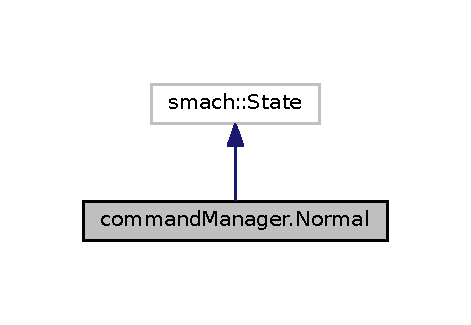
\includegraphics[width=226pt]{classcommandManager_1_1Normal__inherit__graph}
\end{center}
\end{figure}


Collaboration diagram for command\+Manager.\+Normal\+:\nopagebreak
\begin{figure}[H]
\begin{center}
\leavevmode
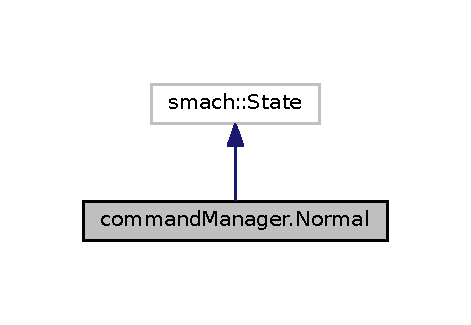
\includegraphics[width=226pt]{classcommandManager_1_1Normal__coll__graph}
\end{center}
\end{figure}
\subsection*{Public Member Functions}
\begin{DoxyCompactItemize}
\item 
def \hyperlink{classcommandManager_1_1Normal_abda69ab53b7d84c2c0c577dcf26f3823}{\+\_\+\+\_\+init\+\_\+\+\_\+} (self)
\item 
def \hyperlink{classcommandManager_1_1Normal_ae95451bab37e817557988c7190bb33bd}{execute} (self, userdata)
\end{DoxyCompactItemize}
\subsection*{Public Attributes}
\begin{DoxyCompactItemize}
\item 
\hyperlink{classcommandManager_1_1Normal_a32e84cf5ac08ffeb9cb1a21d4b484a32}{rate}
\end{DoxyCompactItemize}
\subsection*{Static Public Attributes}
\begin{DoxyCompactItemize}
\item 
\hyperlink{classcommandManager_1_1Normal_a5ebc9e1cc3847edb576acedd01487023}{counter}
\begin{DoxyCompactList}\small\item\em Counter variable to check the number of iteration of the N\+O\+R\+M\+AL state in order to move to S\+L\+E\+EP state after a certain number. \end{DoxyCompactList}\item 
\hyperlink{classcommandManager_1_1Normal_a160432e70539a4ac4dd4a5bf733824a3}{pos} = rooms.\+generate\+\_\+rand\+\_\+pos()
\end{DoxyCompactItemize}


\subsection{Detailed Description}
\begin{DoxyVerb}This class defines the NORMAL state of the FSM. In particular It sends random position to the navigation_action server
and it checks whether a ball is detected in order to move to PLAY state.
Otherwise after some iterations it goes in SLEEP mode \end{DoxyVerb}
 

\subsection{Constructor \& Destructor Documentation}
\index{command\+Manager\+::\+Normal@{command\+Manager\+::\+Normal}!\+\_\+\+\_\+init\+\_\+\+\_\+@{\+\_\+\+\_\+init\+\_\+\+\_\+}}
\index{\+\_\+\+\_\+init\+\_\+\+\_\+@{\+\_\+\+\_\+init\+\_\+\+\_\+}!command\+Manager\+::\+Normal@{command\+Manager\+::\+Normal}}
\subsubsection[{\texorpdfstring{\+\_\+\+\_\+init\+\_\+\+\_\+(self)}{__init__(self)}}]{\setlength{\rightskip}{0pt plus 5cm}def command\+Manager.\+Normal.\+\_\+\+\_\+init\+\_\+\+\_\+ (
\begin{DoxyParamCaption}
\item[{}]{self}
\end{DoxyParamCaption}
)}\hypertarget{classcommandManager_1_1Normal_abda69ab53b7d84c2c0c577dcf26f3823}{}\label{classcommandManager_1_1Normal_abda69ab53b7d84c2c0c577dcf26f3823}


\subsection{Member Function Documentation}
\index{command\+Manager\+::\+Normal@{command\+Manager\+::\+Normal}!execute@{execute}}
\index{execute@{execute}!command\+Manager\+::\+Normal@{command\+Manager\+::\+Normal}}
\subsubsection[{\texorpdfstring{execute(self, userdata)}{execute(self, userdata)}}]{\setlength{\rightskip}{0pt plus 5cm}def command\+Manager.\+Normal.\+execute (
\begin{DoxyParamCaption}
\item[{}]{self, }
\item[{}]{userdata}
\end{DoxyParamCaption}
)}\hypertarget{classcommandManager_1_1Normal_ae95451bab37e817557988c7190bb33bd}{}\label{classcommandManager_1_1Normal_ae95451bab37e817557988c7190bb33bd}


\subsection{Member Data Documentation}
\index{command\+Manager\+::\+Normal@{command\+Manager\+::\+Normal}!counter@{counter}}
\index{counter@{counter}!command\+Manager\+::\+Normal@{command\+Manager\+::\+Normal}}
\subsubsection[{\texorpdfstring{counter}{counter}}]{\setlength{\rightskip}{0pt plus 5cm}command\+Manager.\+Normal.\+counter\hspace{0.3cm}{\ttfamily [static]}}\hypertarget{classcommandManager_1_1Normal_a5ebc9e1cc3847edb576acedd01487023}{}\label{classcommandManager_1_1Normal_a5ebc9e1cc3847edb576acedd01487023}


Counter variable to check the number of iteration of the N\+O\+R\+M\+AL state in order to move to S\+L\+E\+EP state after a certain number. 

\index{command\+Manager\+::\+Normal@{command\+Manager\+::\+Normal}!pos@{pos}}
\index{pos@{pos}!command\+Manager\+::\+Normal@{command\+Manager\+::\+Normal}}
\subsubsection[{\texorpdfstring{pos}{pos}}]{\setlength{\rightskip}{0pt plus 5cm}command\+Manager.\+Normal.\+pos = rooms.\+generate\+\_\+rand\+\_\+pos()\hspace{0.3cm}{\ttfamily [static]}}\hypertarget{classcommandManager_1_1Normal_a160432e70539a4ac4dd4a5bf733824a3}{}\label{classcommandManager_1_1Normal_a160432e70539a4ac4dd4a5bf733824a3}
\index{command\+Manager\+::\+Normal@{command\+Manager\+::\+Normal}!rate@{rate}}
\index{rate@{rate}!command\+Manager\+::\+Normal@{command\+Manager\+::\+Normal}}
\subsubsection[{\texorpdfstring{rate}{rate}}]{\setlength{\rightskip}{0pt plus 5cm}command\+Manager.\+Normal.\+rate}\hypertarget{classcommandManager_1_1Normal_a32e84cf5ac08ffeb9cb1a21d4b484a32}{}\label{classcommandManager_1_1Normal_a32e84cf5ac08ffeb9cb1a21d4b484a32}


The documentation for this class was generated from the following file\+:\begin{DoxyCompactItemize}
\item 
/home/francescotesta/experimental\+\_\+ws/src/final\+\_\+assignment/scripts/\hyperlink{commandManager_8py}{command\+Manager.\+py}\end{DoxyCompactItemize}

\hypertarget{classcommandManager_1_1Play}{}\section{command\+Manager.\+Play Class Reference}
\label{classcommandManager_1_1Play}\index{command\+Manager.\+Play@{command\+Manager.\+Play}}


Inheritance diagram for command\+Manager.\+Play\+:\nopagebreak
\begin{figure}[H]
\begin{center}
\leavevmode
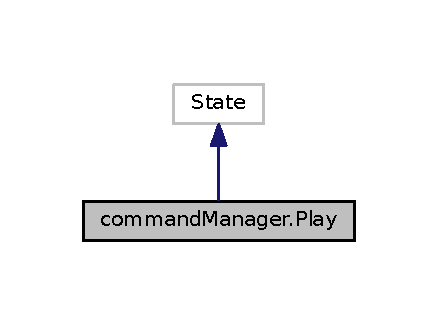
\includegraphics[width=210pt]{classcommandManager_1_1Play__inherit__graph}
\end{center}
\end{figure}


Collaboration diagram for command\+Manager.\+Play\+:\nopagebreak
\begin{figure}[H]
\begin{center}
\leavevmode
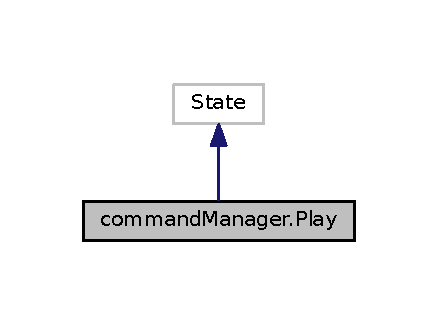
\includegraphics[width=210pt]{classcommandManager_1_1Play__coll__graph}
\end{center}
\end{figure}
\subsection*{Public Member Functions}
\begin{DoxyCompactItemize}
\item 
def \hyperlink{classcommandManager_1_1Play_a4bc5c3700d80432b4dd09b163f210540}{\+\_\+\+\_\+init\+\_\+\+\_\+} (self)
\item 
def \hyperlink{classcommandManager_1_1Play_a2ec6a287ce47f3f6c08c76cc452cf4d3}{execute} (self, userdata)
\end{DoxyCompactItemize}
\subsection*{Public Attributes}
\begin{DoxyCompactItemize}
\item 
\hyperlink{classcommandManager_1_1Play_a34aba8df5dfec3560f194934b7e377ad}{rate}
\end{DoxyCompactItemize}
\subsection*{Static Public Attributes}
\begin{DoxyCompactItemize}
\item 
\hyperlink{classcommandManager_1_1Play_a0999085c98a27adf5b79df2691a7e222}{counter}
\begin{DoxyCompactList}\small\item\em Variable to count the time pass. \end{DoxyCompactList}\item 
\hyperlink{classcommandManager_1_1Play_a0cd6441e9cc0ec9ec7acb974b5b1354e}{position} = rooms.\+get\+\_\+room\+\_\+position(\char`\"{}Home\char`\"{})
\end{DoxyCompactItemize}


\subsection{Detailed Description}
\begin{DoxyVerb}Class that defines the PLAY state. 
 It move the robot in X Y location and then asks to go back to the user.\end{DoxyVerb}
 

\subsection{Constructor \& Destructor Documentation}
\index{command\+Manager\+::\+Play@{command\+Manager\+::\+Play}!\+\_\+\+\_\+init\+\_\+\+\_\+@{\+\_\+\+\_\+init\+\_\+\+\_\+}}
\index{\+\_\+\+\_\+init\+\_\+\+\_\+@{\+\_\+\+\_\+init\+\_\+\+\_\+}!command\+Manager\+::\+Play@{command\+Manager\+::\+Play}}
\subsubsection[{\texorpdfstring{\+\_\+\+\_\+init\+\_\+\+\_\+(self)}{__init__(self)}}]{\setlength{\rightskip}{0pt plus 5cm}def command\+Manager.\+Play.\+\_\+\+\_\+init\+\_\+\+\_\+ (
\begin{DoxyParamCaption}
\item[{}]{self}
\end{DoxyParamCaption}
)}\hypertarget{classcommandManager_1_1Play_a4bc5c3700d80432b4dd09b163f210540}{}\label{classcommandManager_1_1Play_a4bc5c3700d80432b4dd09b163f210540}
\begin{DoxyVerb}Class that defines the PLAY state. 
 It move the robot in X Y location and then asks to go back to the user.\end{DoxyVerb}
 

\subsection{Member Function Documentation}
\index{command\+Manager\+::\+Play@{command\+Manager\+::\+Play}!execute@{execute}}
\index{execute@{execute}!command\+Manager\+::\+Play@{command\+Manager\+::\+Play}}
\subsubsection[{\texorpdfstring{execute(self, userdata)}{execute(self, userdata)}}]{\setlength{\rightskip}{0pt plus 5cm}def command\+Manager.\+Play.\+execute (
\begin{DoxyParamCaption}
\item[{}]{self, }
\item[{}]{userdata}
\end{DoxyParamCaption}
)}\hypertarget{classcommandManager_1_1Play_a2ec6a287ce47f3f6c08c76cc452cf4d3}{}\label{classcommandManager_1_1Play_a2ec6a287ce47f3f6c08c76cc452cf4d3}


\subsection{Member Data Documentation}
\index{command\+Manager\+::\+Play@{command\+Manager\+::\+Play}!counter@{counter}}
\index{counter@{counter}!command\+Manager\+::\+Play@{command\+Manager\+::\+Play}}
\subsubsection[{\texorpdfstring{counter}{counter}}]{\setlength{\rightskip}{0pt plus 5cm}command\+Manager.\+Play.\+counter\hspace{0.3cm}{\ttfamily [static]}}\hypertarget{classcommandManager_1_1Play_a0999085c98a27adf5b79df2691a7e222}{}\label{classcommandManager_1_1Play_a0999085c98a27adf5b79df2691a7e222}


Variable to count the time pass. 

\index{command\+Manager\+::\+Play@{command\+Manager\+::\+Play}!position@{position}}
\index{position@{position}!command\+Manager\+::\+Play@{command\+Manager\+::\+Play}}
\subsubsection[{\texorpdfstring{position}{position}}]{\setlength{\rightskip}{0pt plus 5cm}command\+Manager.\+Play.\+position = rooms.\+get\+\_\+room\+\_\+position(\char`\"{}Home\char`\"{})\hspace{0.3cm}{\ttfamily [static]}}\hypertarget{classcommandManager_1_1Play_a0cd6441e9cc0ec9ec7acb974b5b1354e}{}\label{classcommandManager_1_1Play_a0cd6441e9cc0ec9ec7acb974b5b1354e}
\index{command\+Manager\+::\+Play@{command\+Manager\+::\+Play}!rate@{rate}}
\index{rate@{rate}!command\+Manager\+::\+Play@{command\+Manager\+::\+Play}}
\subsubsection[{\texorpdfstring{rate}{rate}}]{\setlength{\rightskip}{0pt plus 5cm}command\+Manager.\+Play.\+rate}\hypertarget{classcommandManager_1_1Play_a34aba8df5dfec3560f194934b7e377ad}{}\label{classcommandManager_1_1Play_a34aba8df5dfec3560f194934b7e377ad}


The documentation for this class was generated from the following file\+:\begin{DoxyCompactItemize}
\item 
/home/francescotesta/experimental\+\_\+ws/src/final\+\_\+assignment/scripts/\hyperlink{commandManager_8py}{command\+Manager.\+py}\end{DoxyCompactItemize}

\hypertarget{classcommandManager_1_1Sleep}{}\section{command\+Manager.\+Sleep Class Reference}
\label{classcommandManager_1_1Sleep}\index{command\+Manager.\+Sleep@{command\+Manager.\+Sleep}}


Inheritance diagram for command\+Manager.\+Sleep\+:\nopagebreak
\begin{figure}[H]
\begin{center}
\leavevmode
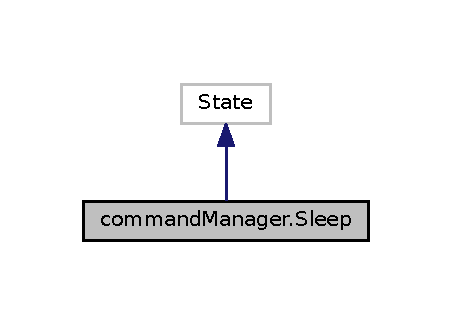
\includegraphics[width=217pt]{classcommandManager_1_1Sleep__inherit__graph}
\end{center}
\end{figure}


Collaboration diagram for command\+Manager.\+Sleep\+:\nopagebreak
\begin{figure}[H]
\begin{center}
\leavevmode
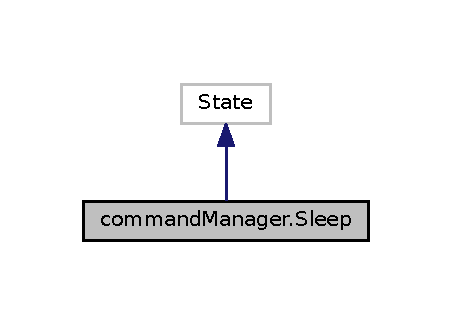
\includegraphics[width=217pt]{classcommandManager_1_1Sleep__coll__graph}
\end{center}
\end{figure}
\subsection*{Public Member Functions}
\begin{DoxyCompactItemize}
\item 
def \hyperlink{classcommandManager_1_1Sleep_aa31bb1cc360e9bb1d723eaf953295268}{\+\_\+\+\_\+init\+\_\+\+\_\+} (self)
\item 
def \hyperlink{classcommandManager_1_1Sleep_a01a1b33499ec3c862bed42a6258b0f12}{execute} (self, userdata)
\end{DoxyCompactItemize}
\subsection*{Public Attributes}
\begin{DoxyCompactItemize}
\item 
\hyperlink{classcommandManager_1_1Sleep_ad1bca2bd2c57109d92089b82fafe23c1}{rate}
\end{DoxyCompactItemize}
\subsection*{Static Public Attributes}
\begin{DoxyCompactItemize}
\item 
\hyperlink{classcommandManager_1_1Sleep_ab64714b4c7c4b5a8824986a8e7af976e}{position} = rooms.\+get\+\_\+room\+\_\+position(\char`\"{}Home\char`\"{})
\end{DoxyCompactItemize}


\subsection{Detailed Description}
\begin{DoxyVerb}It defines the SLEEP state where the robot sleeps for a random period of time.
Then it makes a request to the move_base action server to go to the home location.
Finally it returns in the NORMAL state\end{DoxyVerb}
 

\subsection{Constructor \& Destructor Documentation}
\index{command\+Manager\+::\+Sleep@{command\+Manager\+::\+Sleep}!\+\_\+\+\_\+init\+\_\+\+\_\+@{\+\_\+\+\_\+init\+\_\+\+\_\+}}
\index{\+\_\+\+\_\+init\+\_\+\+\_\+@{\+\_\+\+\_\+init\+\_\+\+\_\+}!command\+Manager\+::\+Sleep@{command\+Manager\+::\+Sleep}}
\subsubsection[{\texorpdfstring{\+\_\+\+\_\+init\+\_\+\+\_\+(self)}{__init__(self)}}]{\setlength{\rightskip}{0pt plus 5cm}def command\+Manager.\+Sleep.\+\_\+\+\_\+init\+\_\+\+\_\+ (
\begin{DoxyParamCaption}
\item[{}]{self}
\end{DoxyParamCaption}
)}\hypertarget{classcommandManager_1_1Sleep_aa31bb1cc360e9bb1d723eaf953295268}{}\label{classcommandManager_1_1Sleep_aa31bb1cc360e9bb1d723eaf953295268}
\begin{DoxyVerb}It defines the SLEEP state where the robot sleeps for a random period of time.
Then it makes a request to the move_base action server to go to the home location.
Finally it returns in the NORMAL state\end{DoxyVerb}
 

\subsection{Member Function Documentation}
\index{command\+Manager\+::\+Sleep@{command\+Manager\+::\+Sleep}!execute@{execute}}
\index{execute@{execute}!command\+Manager\+::\+Sleep@{command\+Manager\+::\+Sleep}}
\subsubsection[{\texorpdfstring{execute(self, userdata)}{execute(self, userdata)}}]{\setlength{\rightskip}{0pt plus 5cm}def command\+Manager.\+Sleep.\+execute (
\begin{DoxyParamCaption}
\item[{}]{self, }
\item[{}]{userdata}
\end{DoxyParamCaption}
)}\hypertarget{classcommandManager_1_1Sleep_a01a1b33499ec3c862bed42a6258b0f12}{}\label{classcommandManager_1_1Sleep_a01a1b33499ec3c862bed42a6258b0f12}


\subsection{Member Data Documentation}
\index{command\+Manager\+::\+Sleep@{command\+Manager\+::\+Sleep}!position@{position}}
\index{position@{position}!command\+Manager\+::\+Sleep@{command\+Manager\+::\+Sleep}}
\subsubsection[{\texorpdfstring{position}{position}}]{\setlength{\rightskip}{0pt plus 5cm}command\+Manager.\+Sleep.\+position = rooms.\+get\+\_\+room\+\_\+position(\char`\"{}Home\char`\"{})\hspace{0.3cm}{\ttfamily [static]}}\hypertarget{classcommandManager_1_1Sleep_ab64714b4c7c4b5a8824986a8e7af976e}{}\label{classcommandManager_1_1Sleep_ab64714b4c7c4b5a8824986a8e7af976e}
\index{command\+Manager\+::\+Sleep@{command\+Manager\+::\+Sleep}!rate@{rate}}
\index{rate@{rate}!command\+Manager\+::\+Sleep@{command\+Manager\+::\+Sleep}}
\subsubsection[{\texorpdfstring{rate}{rate}}]{\setlength{\rightskip}{0pt plus 5cm}command\+Manager.\+Sleep.\+rate}\hypertarget{classcommandManager_1_1Sleep_ad1bca2bd2c57109d92089b82fafe23c1}{}\label{classcommandManager_1_1Sleep_ad1bca2bd2c57109d92089b82fafe23c1}


The documentation for this class was generated from the following file\+:\begin{DoxyCompactItemize}
\item 
/home/francescotesta/experimental\+\_\+ws/src/final\+\_\+assignment/scripts/\hyperlink{commandManager_8py}{command\+Manager.\+py}\end{DoxyCompactItemize}

\chapter{File Documentation}
\hypertarget{ballDetection_8py}{}\section{/home/experimental\+\_\+ws/experimental\+\_\+ws/src/assignment2/scripts/ball\+Detection.py File Reference}
\label{ballDetection_8py}\index{/home/experimental\+\_\+ws/experimental\+\_\+ws/src/assignment2/scripts/ball\+Detection.\+py@{/home/experimental\+\_\+ws/experimental\+\_\+ws/src/assignment2/scripts/ball\+Detection.\+py}}
\subsection*{Classes}
\begin{DoxyCompactItemize}
\item 
class \hyperlink{classballDetection_1_1image__feature}{ball\+Detection.\+image\+\_\+feature}
\end{DoxyCompactItemize}
\subsection*{Namespaces}
\begin{DoxyCompactItemize}
\item 
 \hyperlink{namespaceballDetection}{ball\+Detection}
\end{DoxyCompactItemize}
\subsection*{Functions}
\begin{DoxyCompactItemize}
\item 
def \hyperlink{namespaceballDetection_a8193b8aef394c20f60fadbaeacdafdc0}{ball\+Detection.\+main} (args)
\end{DoxyCompactItemize}
\subsection*{Variables}
\begin{DoxyCompactItemize}
\item 
bool \hyperlink{namespaceballDetection_a647c27a849ab906ef614cb5026275f43}{ball\+Detection.\+V\+E\+R\+B\+O\+SE} = False
\end{DoxyCompactItemize}

\hypertarget{commandManager_8py}{}\section{/home/francescotesta/experimental\+\_\+ws/src/final\+\_\+assignment/scripts/command\+Manager.py File Reference}
\label{commandManager_8py}\index{/home/francescotesta/experimental\+\_\+ws/src/final\+\_\+assignment/scripts/command\+Manager.\+py@{/home/francescotesta/experimental\+\_\+ws/src/final\+\_\+assignment/scripts/command\+Manager.\+py}}


This script is a node which is the core of the entier project.  


\subsection*{Classes}
\begin{DoxyCompactItemize}
\item 
class \hyperlink{classcommandManager_1_1Normal}{command\+Manager.\+Normal}
\item 
class \hyperlink{classcommandManager_1_1Sleep}{command\+Manager.\+Sleep}
\item 
class \hyperlink{classcommandManager_1_1Play}{command\+Manager.\+Play}
\item 
class \hyperlink{classcommandManager_1_1Track}{command\+Manager.\+Track}
\item 
class \hyperlink{classcommandManager_1_1Find}{command\+Manager.\+Find}
\end{DoxyCompactItemize}
\subsection*{Namespaces}
\begin{DoxyCompactItemize}
\item 
 \hyperlink{namespacecommandManager}{command\+Manager}
\end{DoxyCompactItemize}
\subsection*{Functions}
\begin{DoxyCompactItemize}
\item 
def \hyperlink{namespacecommandManager_a2310383d56755f0a09a75b1a92130e21}{command\+Manager.\+U\+Icallback} (data)
\begin{DoxyCompactList}\small\item\em Callback mathod of the U\+Isubscriber which handels the commands sent by the user. \end{DoxyCompactList}\item 
def \hyperlink{namespacecommandManager_aa96fd2ed94c8c1168e09ced4015dcb1b}{command\+Manager.\+new\+Room\+Detected} (color)
\begin{DoxyCompactList}\small\item\em Callback function of the new\+Room\+Sub subscriber which recives the color of the new detected room. \end{DoxyCompactList}\item 
def \hyperlink{namespacecommandManager_af8e54858c65310eb1e131529bf200516}{command\+Manager.\+move\+\_\+base\+\_\+go\+\_\+to} (x, y)
\begin{DoxyCompactList}\small\item\em Method which prepares and send the goal to the move\+\_\+base action server. \end{DoxyCompactList}\item 
def \hyperlink{namespacecommandManager_ae8b570eb4bf393859bc74c9cb5fe125f}{command\+Manager.\+main} ()
\end{DoxyCompactItemize}
\subsection*{Variables}
\begin{DoxyCompactItemize}
\item 
dictionary \hyperlink{namespacecommandManager_a3c82d03952562f9cf96be2e80ae059a3}{command\+Manager.\+control\+\_\+variables}
\begin{DoxyCompactList}\small\item\em Dictionary which contains flags and global variables. \end{DoxyCompactList}\item 
\hyperlink{namespacecommandManager_ad81f5cdd9bf18b67989c77a2329b9e28}{command\+Manager.\+client} = actionlib.\+Simple\+Action\+Client(\textquotesingle{}move\+\_\+base\textquotesingle{},Move\+Base\+Action)
\begin{DoxyCompactList}\small\item\em Initialization of the move\+\_\+base client in order to assign target position to the move\+\_\+base action server. \end{DoxyCompactList}\item 
\hyperlink{namespacecommandManager_a5cf709943d61e92e0ce4c1652403ae8d}{command\+Manager.\+room\+D\+\_\+pub} = rospy.\+Publisher(\textquotesingle{}start\+RD\textquotesingle{}, Bool, queue\+\_\+size=10)
\begin{DoxyCompactList}\small\item\em Publisher to the start\+RD topic which allows to enable/disable the room detector. \end{DoxyCompactList}\item 
\hyperlink{namespacecommandManager_a868809e1f6a79e7b7ce5ea405e978d48}{command\+Manager.\+rooms} = Rooms()
\begin{DoxyCompactList}\small\item\em Object of the class \hyperlink{namespaceRooms}{Rooms} necessary for the knowledge representation of the environment. \end{DoxyCompactList}\end{DoxyCompactItemize}


\subsection{Detailed Description}
This script is a node which is the core of the entier project. 

And implement a finite state machine with five states which are described in the R\+E\+A\+D\+ME file. It manages the messages comming from other nodes and R\+OS packeges. \begin{DoxySeeAlso}{See also}
\hyperlink{namespaceroomDetector}{room\+Detector} 

\hyperlink{namespaceUI}{UI} 

\hyperlink{namespacetrack}{track} 
\end{DoxySeeAlso}

\hypertarget{cvtest_8py}{}\section{/home/experimental\+\_\+ws/experimental\+\_\+ws/src/assignment2/scripts/cvtest.py File Reference}
\label{cvtest_8py}\index{/home/experimental\+\_\+ws/experimental\+\_\+ws/src/assignment2/scripts/cvtest.\+py@{/home/experimental\+\_\+ws/experimental\+\_\+ws/src/assignment2/scripts/cvtest.\+py}}
\subsection*{Classes}
\begin{DoxyCompactItemize}
\item 
class \hyperlink{classcvtest_1_1image__feature}{cvtest.\+image\+\_\+feature}
\end{DoxyCompactItemize}
\subsection*{Namespaces}
\begin{DoxyCompactItemize}
\item 
 \hyperlink{namespacecvtest}{cvtest}
\end{DoxyCompactItemize}
\subsection*{Functions}
\begin{DoxyCompactItemize}
\item 
def \hyperlink{namespacecvtest_ae154ff2084b8756ce8c727d4308e16e5}{cvtest.\+main} (args)
\end{DoxyCompactItemize}
\subsection*{Variables}
\begin{DoxyCompactItemize}
\item 
bool \hyperlink{namespacecvtest_a77dc49644bd9f436671cd8f839604a45}{cvtest.\+V\+E\+R\+B\+O\+SE} = False
\end{DoxyCompactItemize}

\hypertarget{go__to__point__ball_8py}{}\section{/home/experimental\+\_\+ws/experimental\+\_\+ws/src/assignment2/scripts/go\+\_\+to\+\_\+point\+\_\+ball.py File Reference}
\label{go__to__point__ball_8py}\index{/home/experimental\+\_\+ws/experimental\+\_\+ws/src/assignment2/scripts/go\+\_\+to\+\_\+point\+\_\+ball.\+py@{/home/experimental\+\_\+ws/experimental\+\_\+ws/src/assignment2/scripts/go\+\_\+to\+\_\+point\+\_\+ball.\+py}}
\subsection*{Namespaces}
\begin{DoxyCompactItemize}
\item 
 \hyperlink{namespacego__to__point__ball}{go\+\_\+to\+\_\+point\+\_\+ball}
\end{DoxyCompactItemize}
\subsection*{Functions}
\begin{DoxyCompactItemize}
\item 
def \hyperlink{namespacego__to__point__ball_a8b53c165c87e66822f50ab5daebc14dc}{go\+\_\+to\+\_\+point\+\_\+ball.\+clbk\+\_\+odom} (msg)
\item 
def \hyperlink{namespacego__to__point__ball_ac5839fd3601d15749a1e1a28939b2c68}{go\+\_\+to\+\_\+point\+\_\+ball.\+change\+\_\+state} (state)
\item 
def \hyperlink{namespacego__to__point__ball_aecbf76a67251ff6a3a0840bb61e1c581}{go\+\_\+to\+\_\+point\+\_\+ball.\+go\+\_\+straight\+\_\+ahead} (des\+\_\+pos)
\item 
def \hyperlink{namespacego__to__point__ball_ab92c8b4240f09ff0b5d960c748ade799}{go\+\_\+to\+\_\+point\+\_\+ball.\+done} ()
\item 
def \hyperlink{namespacego__to__point__ball_ab0e05a6be4adc81f80b5635d9bd692d1}{go\+\_\+to\+\_\+point\+\_\+ball.\+planning} (goal)
\item 
def \hyperlink{namespacego__to__point__ball_a4d4c016b6bb12c612710a2d39ade3465}{go\+\_\+to\+\_\+point\+\_\+ball.\+main} ()
\end{DoxyCompactItemize}
\subsection*{Variables}
\begin{DoxyCompactItemize}
\item 
\hyperlink{namespacego__to__point__ball_aa399e57145dd0af7eefcd5fab4174fe9}{go\+\_\+to\+\_\+point\+\_\+ball.\+position\+\_\+} = Point()
\item 
\hyperlink{namespacego__to__point__ball_a03f1d8b257a2ae3d173a18c3fc2f8602}{go\+\_\+to\+\_\+point\+\_\+ball.\+pose\+\_\+} = Pose()
\item 
int \hyperlink{namespacego__to__point__ball_a74d8ca28c507d35baf1ea8e8f9595a78}{go\+\_\+to\+\_\+point\+\_\+ball.\+yaw\+\_\+} = 0
\item 
int \hyperlink{namespacego__to__point__ball_a0028df70b94b4041119cceba5e5aa79d}{go\+\_\+to\+\_\+point\+\_\+ball.\+state\+\_\+} = 0
\item 
\hyperlink{namespacego__to__point__ball_ac81a8393fb253c9e0b7255f779f16884}{go\+\_\+to\+\_\+point\+\_\+ball.\+desired\+\_\+position\+\_\+} = Point()
\item 
int \hyperlink{namespacego__to__point__ball_acc228d72c1ee47a43061e3563ac20d5c}{go\+\_\+to\+\_\+point\+\_\+ball.\+yaw\+\_\+precision\+\_\+} = math.\+pi/9
\item 
int \hyperlink{namespacego__to__point__ball_a1985c69cf8534ba0bd2c6080f788a992}{go\+\_\+to\+\_\+point\+\_\+ball.\+yaw\+\_\+precision\+\_\+2\+\_\+} = math.\+pi/90
\item 
float \hyperlink{namespacego__to__point__ball_a9a02c8ca89a09909111972ec4fd317ca}{go\+\_\+to\+\_\+point\+\_\+ball.\+dist\+\_\+precision\+\_\+} = 0.\+1
\item 
float \hyperlink{namespacego__to__point__ball_aac67ecb6c41141092b1ccaba4b537afc}{go\+\_\+to\+\_\+point\+\_\+ball.\+kp\+\_\+a} = 3.\+0
\item 
float \hyperlink{namespacego__to__point__ball_aeb49969b88b7ca77d9abdeae42cb1964}{go\+\_\+to\+\_\+point\+\_\+ball.\+kp\+\_\+d} = 0.\+5
\item 
float \hyperlink{namespacego__to__point__ball_aa5173a26f3502ea035d7c563bbf1fb05}{go\+\_\+to\+\_\+point\+\_\+ball.\+ub\+\_\+a} = 0.\+6
\item 
float \hyperlink{namespacego__to__point__ball_ae6440cb2a8ea6e8e7d2327cb4cd12dd3}{go\+\_\+to\+\_\+point\+\_\+ball.\+lb\+\_\+a} = -\/0.\+5
\item 
float \hyperlink{namespacego__to__point__ball_a1dabe6f24f898fa6f5303959917de757}{go\+\_\+to\+\_\+point\+\_\+ball.\+ub\+\_\+d} = 2.\+0
\item 
float \hyperlink{namespacego__to__point__ball_a176944c73499ce72fa754c7e1a6d138d}{go\+\_\+to\+\_\+point\+\_\+ball.\+z\+\_\+back} = 0.\+25
\item 
\hyperlink{namespacego__to__point__ball_a00b95c7141b558cd4466ca89d7c81640}{go\+\_\+to\+\_\+point\+\_\+ball.\+pub} = None
\item 
\hyperlink{namespacego__to__point__ball_ae3016b9645d9bd2b863a34a30115a6af}{go\+\_\+to\+\_\+point\+\_\+ball.\+pubz} = None
\item 
\hyperlink{namespacego__to__point__ball_a9ac8c67ea55b320e5eb2bdf665173ffa}{go\+\_\+to\+\_\+point\+\_\+ball.\+act\+\_\+s} = None
\end{DoxyCompactItemize}

\hypertarget{navigation__action_8py}{}\section{/home/experimental\+\_\+ws/experimental\+\_\+ws/src/assignment2/scripts/navigation\+\_\+action.py File Reference}
\label{navigation__action_8py}\index{/home/experimental\+\_\+ws/experimental\+\_\+ws/src/assignment2/scripts/navigation\+\_\+action.\+py@{/home/experimental\+\_\+ws/experimental\+\_\+ws/src/assignment2/scripts/navigation\+\_\+action.\+py}}
\subsection*{Namespaces}
\begin{DoxyCompactItemize}
\item 
 \hyperlink{namespacenavigation__action}{navigation\+\_\+action}
\end{DoxyCompactItemize}
\subsection*{Functions}
\begin{DoxyCompactItemize}
\item 
def \hyperlink{namespacenavigation__action_a5843780136ed9def4e6c383d936ba03a}{navigation\+\_\+action.\+clbk\+\_\+odom} (msg)
\begin{DoxyCompactList}\small\item\em callbacks \end{DoxyCompactList}\item 
def \hyperlink{namespacenavigation__action_a6d442ed74e58d2364dc836bf9070e294}{navigation\+\_\+action.\+change\+\_\+state} (state)
\item 
def \hyperlink{namespacenavigation__action_a3d7bfdf0b3a4ceae6de2da2a2ca9216b}{navigation\+\_\+action.\+normalize\+\_\+angle} (angle)
\item 
def \hyperlink{namespacenavigation__action_a66a81926b4ce0cf801c2a1e947dd2405}{navigation\+\_\+action.\+fix\+\_\+yaw} (des\+\_\+pos)
\item 
def \hyperlink{namespacenavigation__action_a5984663372b3695a8566d9ab2b149728}{navigation\+\_\+action.\+go\+\_\+straight\+\_\+ahead} (des\+\_\+pos)
\item 
def \hyperlink{namespacenavigation__action_a05d5b3c910a9327eceb1628bb0696e40}{navigation\+\_\+action.\+done} ()
\item 
def \hyperlink{namespacenavigation__action_a2b437adab0003dc13c8703a505ba0640}{navigation\+\_\+action.\+planning} (goal)
\begin{DoxyCompactList}\small\item\em callback of the action server \end{DoxyCompactList}\item 
def \hyperlink{namespacenavigation__action_a2203bb3f38935f8a73b3ef443dd4eec1}{navigation\+\_\+action.\+main} ()
\end{DoxyCompactItemize}
\subsection*{Variables}
\begin{DoxyCompactItemize}
\item 
\hyperlink{namespacenavigation__action_aa53bb3e42cba75b4faece7677fdf8b1d}{navigation\+\_\+action.\+position\+\_\+} = Point()
\begin{DoxyCompactList}\small\item\em robot state variables \end{DoxyCompactList}\item 
\hyperlink{namespacenavigation__action_ad906a8ccc8be8e7aac7662be3092c3b7}{navigation\+\_\+action.\+pose\+\_\+} = Pose()
\item 
int \hyperlink{namespacenavigation__action_aa356f2a5947d276649face9801529b11}{navigation\+\_\+action.\+yaw\+\_\+} = 0
\item 
int \hyperlink{namespacenavigation__action_ac6656a4827fb720e3c7a7224940626d2}{navigation\+\_\+action.\+state\+\_\+} = 0
\begin{DoxyCompactList}\small\item\em machine state \end{DoxyCompactList}\item 
\hyperlink{namespacenavigation__action_a7ce69adc83a1ee3d37d5e3c6e0e72e32}{navigation\+\_\+action.\+desired\+\_\+position\+\_\+} = Point()
\begin{DoxyCompactList}\small\item\em goal \end{DoxyCompactList}\item 
\hyperlink{namespacenavigation__action_a5258daa88a84ac3fae37a796753c3a6f}{navigation\+\_\+action.\+z}
\item 
int \hyperlink{namespacenavigation__action_a405244594bb4eea456e03e5b095d3869}{navigation\+\_\+action.\+yaw\+\_\+precision\+\_\+} = math.\+pi/9
\begin{DoxyCompactList}\small\item\em parameters \end{DoxyCompactList}\item 
int \hyperlink{namespacenavigation__action_a8ff0e6466c43c2a149fb09b9678d56bf}{navigation\+\_\+action.\+yaw\+\_\+precision\+\_\+2\+\_\+} = math.\+pi/90
\item 
float \hyperlink{namespacenavigation__action_ae84ae6794723578c0bda3eb07d0f1387}{navigation\+\_\+action.\+dist\+\_\+precision\+\_\+} = 0.\+1
\item 
float \hyperlink{namespacenavigation__action_a88d77c73344c091f0e27e30f34b149cc}{navigation\+\_\+action.\+kp\+\_\+a} = 3.\+0
\item 
float \hyperlink{namespacenavigation__action_a34478a1ef79cccac170cae8f045a4018}{navigation\+\_\+action.\+kp\+\_\+d} = 0.\+2
\begin{DoxyCompactList}\small\item\em In R\+OS Noetic, it may be necessary to change the sign of this proportional controller. \end{DoxyCompactList}\item 
float \hyperlink{namespacenavigation__action_a2949c425c74dfbe48d976545b4f4db9d}{navigation\+\_\+action.\+ub\+\_\+a} = 0.\+6
\item 
float \hyperlink{namespacenavigation__action_aa1239a696c81960bbb147a15f3f3bd87}{navigation\+\_\+action.\+lb\+\_\+a} = -\/0.\+5
\item 
float \hyperlink{namespacenavigation__action_aad75661fd33d72b125133a1898175d4b}{navigation\+\_\+action.\+ub\+\_\+d} = 0.\+6
\item 
\hyperlink{namespacenavigation__action_a534f03fffb29fa18e1e2f01c2e99ac90}{navigation\+\_\+action.\+pub} = None
\begin{DoxyCompactList}\small\item\em publisher \end{DoxyCompactList}\item 
\hyperlink{namespacenavigation__action_a0ff6186f4b199de2bb1fff9bdd2ad110}{navigation\+\_\+action.\+act\+\_\+s} = None
\begin{DoxyCompactList}\small\item\em action\+\_\+server \end{DoxyCompactList}\item 
\hyperlink{namespacenavigation__action_a0d7ef71fc2d73b266e305aaca8a1330a}{navigation\+\_\+action.\+joint\+\_\+pub} = rospy.\+Publisher(\char`\"{}joint\+\_\+head\+\_\+controller/command\char`\"{},Float64,queue\+\_\+size=1)
\begin{DoxyCompactList}\small\item\em Publisher. \end{DoxyCompactList}\end{DoxyCompactItemize}

%--- End generated contents ---

% Index
\backmatter
\newpage
\phantomsection
\clearemptydoublepage
\addcontentsline{toc}{chapter}{Index}
\printindex

\end{document}
